\chapter{Balancing Safety and Freedom for the User: Intervention as Planning and Human-aware Intervention}
\label{chap:ch5}
When working in an unfamiliar online environment,  it can be helpful to have an observer that can intervene and guide a user toward a desirable outcome while avoiding undesirable outcomes or frustration.
The {\em Intervention Problem} is deciding when to intervene in order to help a user.
The Intervention Problem is similar to, but distinct from Plan Recognition because the observer must not only recognize the intended goals of a user but also when to intervene to help the user, but also to only intervene when necessary.
We formalize a family of Intervention Problems and show how these problems can be solved using a combination of Plan Recognition methods and classification techniques to decide whether to intervene.
The dimensions of the Intervention Problem presented in this chapter are summarized in Table~\ref{tab:dim3}

\begin{table}[ptb]
\begin{tabular}{|l|l|}
\hline
\textbf{Dimension} & \textbf{Domain Specific Properties} \\ \hline
Actors in the environment & User, Competitor (optional), Observer \\ \hline
Goals hidden to the observer & \begin{tabular}[c]{@{}l@{}}User's goal not hidden\\ One or more known undesirable states\end{tabular} \\ \hline
Types of observations & The user's and the competitor's (if present) actions \\ \hline
Noise in observations & None \\ \hline
Intervention recovery & Offer helpful hint \\ \hline
\end{tabular}
\caption{Dimensions of the Unsafe Suffix Recognition Problem}
\label{tab:dim3}
\end{table}


We characterize the observer’s decision space as an Intervention Graph and 
construct it using an ``Intervention as Classical Planning'' approach to generate potential suffixes of partially executed plans.
We extract domain-independent features from this graph and extend several Plan Recognition benchmarks to evaluate this approach.
For our benchmarks, the learned models dominate three recent Plan Recognition approaches.
We then generalize these results to Human-Aware Intervention, 
where the observer must decide in real time whether to intervene for human users solving a cognitively engaging puzzle.
Using a revised feature set more appropriate to human behavior, 
we produce a learned model to recognize when a human user is about to trigger an undesirable outcome. 
We perform a human-subject study to evaluate the Human-Aware Intervention.
We find that the revised model also dominates existing Plan Recognition algorithms in predicting Human-Aware Intervention.


%===========================================================================================================
%%===========================================================================================================
\section{Introduction}
\noindent Even the best plan can go wrong. 
Dangers arise from failing to execute a plan correctly or as a result of actions executed by a nefarious agent. 
Consider route planning where a driver is unaware of upcoming road damage or a traffic jam. 
Or consider cyber-security where a user is unaware of an unsafe hyperlink. 
In both, plans achieving the desirable goal have similar prefixes to those that result in undesirable outcomes.
Suppose an observer watches the actions of a user working in a risky environment where plans may be subverted to reach an undesirable outcome. 
We study the problem of how the observer decides whether to intervene if the user appears to need help or the user is about to take an action that leads to an undesirable outcome.

We introduce \textit{Plan Intervention} as a new computational problem and relate it to plan recognition. 
To intervene, the observer needs to make a decision whether or not the user's likely plan will avoid the undesirable state. 
Thus, it is possible to argue that if the observer implements an existing state-of-the-art plan recognition algorithm (e.g., Plan Recognition as Planning \cite{ramirez2009plan}), then intervention can take place when the likely goal of the recognized plan satisfies the undesirable state. 
We show that the Intervention Problem carries subtleties that the state-of-the-art Plan Recognition Algorithms are not yet able to handle.
We propose two complementary solutions for Plan Intervention: (1) Unsafe Suffix Intervention and (2) Human-aware Intervention. 
We show that these two complementary solutions dominate state-of-the-art plan recognition algorithms in correctly recognizing when intervention is required.

For intervention, giving goal priors as required for goal/plan recognition is difficult because certain facts about the domain are hidden to the user and unintended goals may be enabled during execution. 
Furthermore, human actors may not construct plans the same way as an automated planner because humans may identify the optimal choice of actions at each time step. 
They may  make mistakes early on during tasks having a steep learning curve. 
Partial knowledge about the domain may preclude the human user from knowing the full effects of his actions or he may not be thinking about the effects at all. 
Therefore, the observer may not always be able to accurately estimate what the users are trying to do.

We study two kinds of Intervention Problems. 
In \emph{Unsafe Suffix Intervention}, the observer uses automated planners to project the remaining suffixes and extract features that can differentiate between safe and unsafe plans. 
We evaluate the recognition accuracy of Unsafe Suffix Intervention on benchmark planning problems. 
In \emph{Human-aware Intervention}, the observer uses the observed partial solution to extract features that can separate safe and unsafe solutions. 
We evaluate the accuracy of Human-aware Intervention on a new Intervention Planning benchmark called Rush Hour.


The contributions of this chapter are:
\begin{itemize}
\item formalizing the online Intervention Problem for determining when the potential of possible damage  of a state warrants interruption.
\item modeling the observer's decision space as an Intervention Graph, which can be constructed explicitly or sampled with an automated planner.
\item defining features to assess the criticality of a state using the Intervention Graph and the sampled plans.
\item extending existing benchmarks by Ramirez~\&~Geffner~ \citeyear{ramirez2009plan, ramirez2010probabilistic} to incorporate Intervention and  evaluating our intervention approach for the extended benchmarks.
\item introducing a new Plan Intervention benchmark domain called \emph{Rush Hour}, where a player moves vehicles arranged on a grid to clear a path for a target vehicle. 
\item formalizing the Human-aware Intervention Problem for the Rush Hour planning task and designing features to estimate the criticality using behavior features derived from the observed partial plan.
\item presenting the results from a human-subjects study where we collected human behavior on Rush Hour.
\item extending an existing plan recognition model to the Intervention Problem and demonstrating that three state-of-the-art plan recognition algorithms do not perform well in Intervention Problems.
\item training and evaluating the classification models using Rush Hour puzzle solutions collected from a human subject experiment and showing that the approach works well for the Rush Hour problem.
\end{itemize}

In this chapter, we first define a general form of the Intervention Problems and introduce three variants: (1) Intervention for a Single User, (2) Intervention in the Presence of a Competitor and (3) Human-aware Intervention. Next, we present approaches for Intervention for a Single User and Intervention in the Presence of a Competitor, both of which use the Intervention Graph and the sampled plans to recognize unsafe suffixes. We evaluate these two approaches against the state-of-the-art plan recognition algorithms on using benchmark planning domains in the benchmarks. Next, we present Human-aware Intervention, that uses machine learning to learn properties of the observed partial plans, as opposed to projecting suffixes, to determine when intervention is required. To evaluate Human-aware Intervention, we introduce a new planning domain called Rush Hour and study how human users solve Rush Hour puzzle as a planning task. We evaluate Human-aware Intervention in the Rush Hour domain compared to state-of-the-art plan recognition algorithms. We conclude the chapter with a discussion on why plan recognition falls short in solving Intervention Problems and present the open questions for future research in designing intervention models.


%%%===========================================================================================================
%%%===========================================================================================================
\section{The Intervention Environment}
\label{sec:distinguishing}
We model {\bf intervention} in environments where a \textit{user} is trying to achieve a desirable goal(s), denoted \desired, while avoiding undesirable outcomes, denoted \undesired.
Note that in contrast to the Intervention Problem discussed in Chapter~\ref{chap:ch4}, the observer has knowledge about \desired and \undesired and must take into account both these goal states in order to make the intervention decision.
Some environments include a \textit{competitor} who may also take actions in the world, but we assume the user is not aware of the competitor's actions, as might happen in cyber-security applications.

We define the \textit{observer} to be the intervening assistant agent. 
An \textit{observer} receives each action and decides whether to forward the action to the execution platform;
this allows the observer to intervene if the action would result in the undesired outcome \undesired.  
The observer holds a history of previous observations $H = (o_1, o_2, \ldots, o_{i-1})$ that indicate the actions executed by the user or competitor.
The user presents the next action as an observation $o_{i}$ to the observer and the observer must decide ``should I intervene?''
This decision necessitates projecting what the observer knows and determining whether the user is about to do something unsafe (\undesired) 
or is moving too far away from a desirable goal (\desired).
We call such a projection a \textit{suffix}.
We denote a single  \textit{suffix} projection as \Suffix and the set of projections as \Suffixes because there will usually be many projections.

  
The intervention models discussed in Chapters~\ref{chap:ch4} and \ref{chap:ch5} emphasize analyzing the remaining suffixes to decide when to intervene.
In Plan Recognition, the observer uses an observation trace $O$ to derive the user's likely plan. $O$ can be either an ordered sequence of actions  \cite{ramirez2009plan,ramirez2010probabilistic} or an ordered sequence of states \cite{sohrabi2016plan}.
In the first form of intervention we present in this chapter, the observer considers the remaining plans (i.e., suffixes) in safe and unsafe partitions to learn to recognize unsafe suffixes in order to help the user avoid \undesired. 
In this case, the observer can help the user by only accepting actions into \historyDef that will safely advance the user toward \desired.
We call the first intervention model, \textit{Unsafe Suffix Intervention}.
In the second form of intervention, the observer learns to recognize that the user is not making progress toward \desired by analyzing the \historyDef when a suffix is not available. In this case,  the observer must offer enough help to \textit{guide} the user toward \desired without giving the solution. 
The second intervention model is particularly useful when the user is a human and it can be difficult to evaluate progress with heuristics like a normal planning agent.
Therefore, we call the second intervention model, \textit{Human-aware Intervention}.
Plan Recognition does not define a method for the user to recover when the observer recognizes a plan leading to \undesired. 
With the proposed intervention models, we address that limitation with two different types of help the observer can offer to the user.

\section{Intervention Examples}

We will present two examples for \textit{Unsafe Suffix Intervention}.
The Grid Navigation domain example is used to illustrate intervention with the user and observer. 
In the grid navigation task illustrated in Figure~\ref{fig:single}, the user navigates from \texttt{W1} to \texttt{Z3} by moving vertically and horizontally and \texttt{Y3} contains a pit the user can not see: \mbox{$\desired=$ \texttt{(AT Z3)}} and \mbox{$\undesired=$ \texttt{(AT Y3)}}. 
Plans corresponding to paths A, B, C are all feasible solutions to the user's planning task. 
However, plans B and C are unsafe because they satisfy $\lbrace\dandu\rbrace$. 

\begin{figure}[tpb]
        \centering{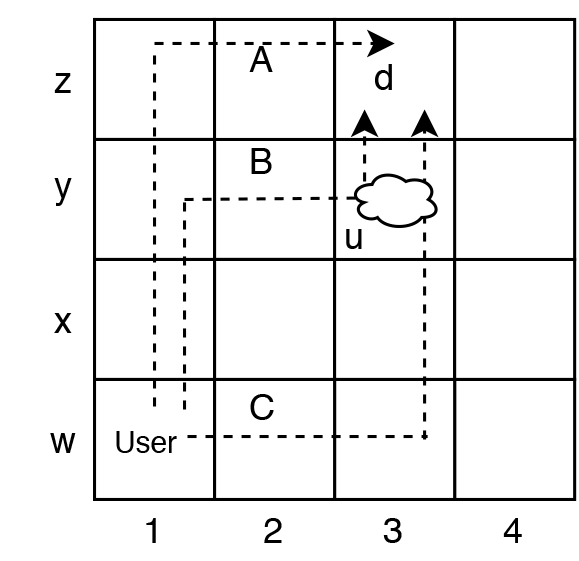
\includegraphics[width=0.3\columnwidth]{img/figure1.jpg}}
         \vspace{-1em}
        \caption{Intervention modeled in the Grid Navigation domain}
        \vspace{-1em}
        \label{fig:single}
\end{figure}


Table~\ref{tab:prpgrid} shows how an observer modeled as an offline Plan Recognition agent will recognize the goals given observations $O$ for the Grid Navigation problem in Figure~\ref{fig:single}. Let us assume that the observer implements the Plan Recognition as Planning algorithm introduced by Ramirez et al. \citeyear{ramirez2010probabilistic} to disambiguate between \undesired and \desired. They show that the most likely goal will be the one that minimizes the cost difference $c(\mathrm{g}|O)-c(\mathrm{g}|\overline{O}), \mathrm{g}\in \lbrace\desired,\undesired\rbrace$. For each incrementally revealed $O$ (shown in columns), assuming uniform goal priors, the observer finds the most likely goal that agrees with $O$. For the cost computation, we assumed that the user is following a satisfising plan to achieve goals. 
It can be seen that for the Grid Navigation example, the observer can not correctly disambiguate between \desired and \undesired. 
More importantly, the final last column satisfies \undesired. At this point, it will be too late for the user to avoid \undesired.
Furthermore, because the observer accepts $O$ as is for Plan Recognition, the observer can not guide the user away from \undesired as the observations are already satisfied in the state.

\begin{table}[t]
\begin{tabular}{|c|l|l|l|l|}
\hline
$O$ & (\textsc{\texttt{move w1 x1}}) & \begin{tabular}[c]{@{}l@{}}(\textsc{\texttt{move w1 x1}}\\ \textsc{\texttt{move x1 y1}})\end{tabular} & \begin{tabular}[c]{@{}l@{}}(\textsc{\texttt{move w1 x1}}\\ \textsc{\texttt{move x1 y1}}\\ \textsc{\texttt{move y1 y2}})\end{tabular} & \begin{tabular}[c]{@{}l@{}}(\textsc{\texttt{move w1 x1}}\\ \textsc{\texttt{move x1 y1}}\\ \textsc{\texttt{move y1 y2}}\\ \textsc{\texttt{move y2 y3}})\end{tabular} \\ \hline
\begin{tabular}[c]{@{}l@{}}$c(\mathrm{u}|O)-c(\mathrm{u}|\overline{O})$\end{tabular} & $4 - 4 = 0$ & $4 - 4 = 0$ & $4 - 4 = 0$ & $4 - 4 = 0$ \\ \hline
\begin{tabular}[c]{@{}l@{}}$c(\mathrm{d}|O)-c(\mathrm{d}|\overline{O})$\end{tabular} & $5 - 5 = 0$ & $5 - 5 = 0$ & $5 - 5 = 0$ & $5 - 5 = 0$ \\ \hline
Most likely goal & No decision & No decision & No decision & Fail \\ \hline
\end{tabular}
\caption{Observer modeled as a Plan Recognition agent for the Grid Navigation example in Figure~\ref{fig:single}}
\label{tab:prpgrid}
\end{table}

\begin{figure}[tpb]
 \centering{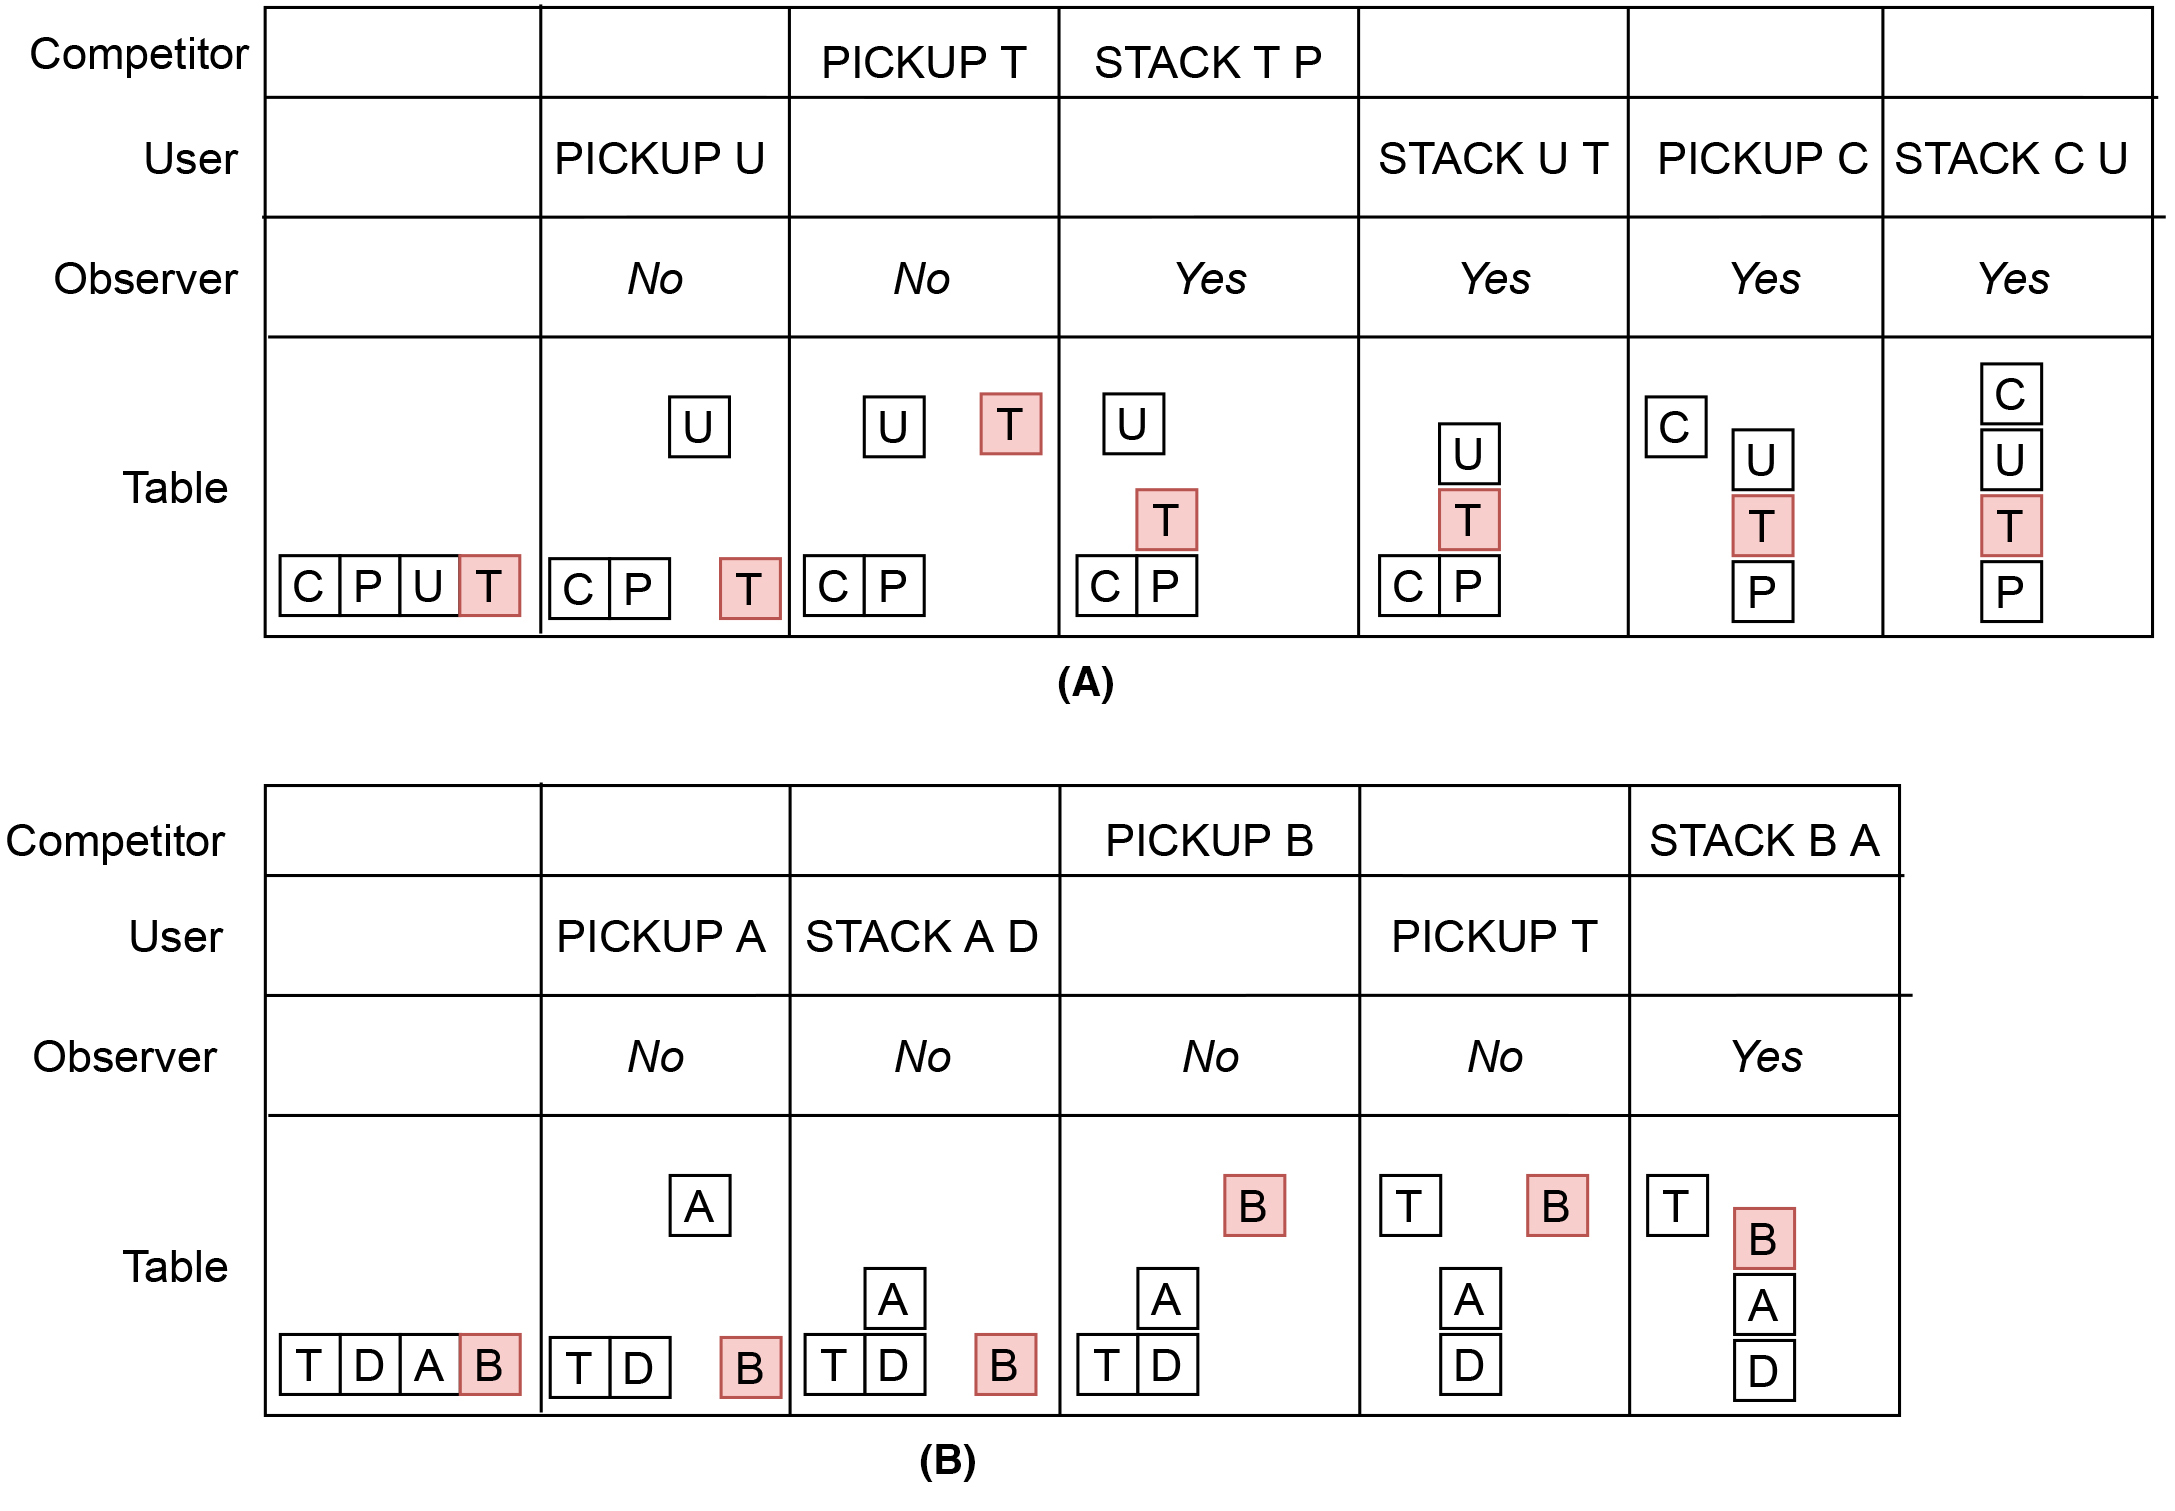
\includegraphics[width=0.7\columnwidth]{img/figure2.jpg}}
   \caption{(A) User and competitor intervention modeled in the Blocks Words domain, where $\undesired=$ (CUT) and $\desired=$ (CUP). (B) User and competitor intervention where $\undesired= $ (BAD) and $\desired= $ (TAD). \\ Initially, all four blocks are on the table. An action in the user or competitor row indicates the Intervention Suffix. The \textit{Yes} label in the observer's row indicates that intervention is required. The \textit{No} label indicates that intervention is not required.}
\label{fig:bw2}
\end{figure}

Now let us consider a situation where there may be some additional agent taking actions in the world.
For example, in a cyber-security application, a second agent may insert malicious code in a file to gain access to privileged information.
More generally, we call this additional agent a competitor, since it is not always the case that they are ``attacking'' a user.
The Blocks Word domain example from Ramirez et al. \citeyear{ramirez2009plan} is used to illustrate intervention with the user, the competitor and the observer. 
In the Intervention Problem illustrated in Figure~\ref{fig:bw2} (A), the competitor's goal $\mathrm{u}=$ $\lbrace$(\texttt{CLEAR C})(\texttt{ON C U})(\texttt{ON U T})$\rbrace$(i.e., CUT) and the user's goal $\mathrm{d}=\lbrace$(\texttt{CLEAR C})(\texttt{ON C U})(\texttt{ON U P})$\rbrace$(i.e., CUP). The user can not recognize the block T (shown in red). The competitor only modify the state of block T and executes actions with the block T. As shown in the first column, initially, all four blocks are on the table. 
Both the user and the competitor incrementally reveal their plans.
The user's and the competitor's rows in Figure~\ref{fig:bw2} (A) show an example reveal sequence from left to right. 
The row for the table shows the resulting states after each reveal.
In this example, the observer needs to recognize that when the competitor reveals \texttt{STACK T P}, it becomes impossible for the user to avoid \undesired. 
However, the user may continue to reveal actions because he can not recognize the post-condition of \texttt{STACK T P}. 
Therefore, any subsequent reveal must also be recognized as unsafe.
The \textit{Yes} labels in the observer's row indicate that intervention is required. 
Note that in the Blocks Words example, \desired and \undesired are distinct enough to disambiguate early.

Table~\ref{tab:prpbw} shows how an observer modeled as an offline Plan Recognition agent will recognize the goals for the Blocks Words problem in Figure~\ref{fig:bw2} (A). Similar to the Grid Navigation example, the Plan Recognition agent implements the Plan Recognition as Planning algorithm introduced by Ramirez et al. \citeyear{ramirez2010probabilistic} to disambiguate between \undesired and \desired. All other assumptions in the Grid Navigation Plan Recognition task also hold in this problem.
It can be seen that in the Blocks Words example the observer disambiguate  \undesired and \desired somewhat better than the Grid Navigation example, because the goals are different enough.
The most likely goal identified by the observer aligns with the Yes/No decisions in Figure~\ref{fig:bw2} (A). 
However, there are still ``observation reveals'' where the observer can not make a clear decision.
In the last reveal, the observer correctly identifies \undesired as the goal. However, the observer can not help the user avoid \undesired in the final reveal because $O$ satisfies \undesired by definition of $O$ in Plan Recognition as Planning. 
With the proposed intervention algorithms, which learn the distinctions between unsafe and safe plans, we hope to improve the intervention recognition accuracy for the observer, while allowing the user some freedom to satisfy \desired avoiding \undesired.
Furthermore, by accepting actions that only help the user advance toward \desired safely into the observation history \historyDef, our intervention algorithm ensures that the user avoids \undesired.

\begin{table}[t]
\resizebox{\textwidth}{!}{%
\begin{tabular}{|c|l|l|l|l|l|l|}
\hline
$O$ & (\textsc{\texttt{PICKUP U}}) & \begin{tabular}[c]{@{}l@{}}(\texttt{\textsc{PICKUP U}}\\ \textsc{\texttt{PICKUP T}})\end{tabular} & \begin{tabular}[c]{@{}l@{}}(\texttt{\textsc{PICKUP U}}\\ \textsc{\texttt{PICKUP T}}\\ \texttt{\textsc{STACK T P}})\end{tabular} & \begin{tabular}[c]{@{}l@{}}(\textsc{\texttt{PICKUP U}}\\ \texttt{\texttt{PICKUP T}}\\ \texttt{\textsc{STACK T P}}\\ \texttt{\textsc{STACK U T}})\end{tabular} & \begin{tabular}[c]{@{}l@{}}(\texttt{\textsc{PICKUP U}}\\ \texttt{\textsc{PICKUP T}}\\ \textsc{\texttt{STACK T P}}\\ \texttt{\textsc{STACK U T}}\\ \texttt{\texttt{PICKUP C}})\end{tabular} & \begin{tabular}[c]{@{}l@{}}(\texttt{\textsc{PICKUP U}}\\ \texttt{\textsc{PICKUP T}}\\ \texttt{\textsc{STACK T P}}\\ \textsc{\texttt{STACK U T}}\\ \texttt{\texttt{PICKUP C}}\\ \texttt{\texttt{STACK C U}})\end{tabular} \\ \hline
\begin{tabular}[c]{@{}l@{}}$c(\mathrm{u}|O)-c(\mathrm{u}|\overline{O})$\end{tabular} & $4 - 4 = 0$ & $8 - 4 = 4$ & $8 - 4 = 4$ & $8 - 4 = 4$ & $8 - 4 = 4$ & $8 - 4 = 4$ \\ \hline
\begin{tabular}[c]{@{}l@{}}$c(\mathrm{d}|O)-c(\mathrm{d}|\overline{O})$\end{tabular} & $4 - 4 = 0$ & $6 - 4 = 2$ & $10 - 4 = 6$ & $16 - 4 = 12$ & $18 - 4 = 14$ & $20 - 4 = 16$ \\ \hline
Most likely goal & No decision & \desired & \undesired & \undesired & \undesired & Fail \\ \hline
\end{tabular}
}%
\caption{Observer modeled as a Plan Recognition agent for the Blocks Words example in Figure~\ref{fig:bw2} (A)}
\label{tab:prpbw}
\end{table}


%%%===========================================================================================================
%%==================================================
%%3 - Intervention Formal Definitions
%%==================================================
\section{Defining Intervention Problems}
\label{sec:intervention-problem}
When intervening in unsafe situations (studied in Sections~\ref{sec:recognizing-unsafe-suffixes}--\ref{sec:evaluating-intervention}), the observer analyzes what we call the  Intervention Suffixes \Suffixes to decide whether they avoid \undesired.
When intervening to help a user (studied in Sections~\ref{sec:human-aware}--\ref{sec:evaluating-hai}), the observer analyzes the history \historyDef to determine if the user is making progress toward \desired (or not) while also avoiding \undesired (or not). 
Both forms are special cases of a more general definition that incorporates the five components (i.e., \desired, \undesired, \historyDef, \presentedAction, and \Suffixes) but emphasizes them differently based on the needs of the application.
In this section we outline our main assumptions (Section~\ref{sec:unsafe-suffix-prelim}), discuss the STRIPS planning model (Section~\ref{sec:models}), discuss an important notion of direct or indirect actions leading to \undesired (Section~\ref{sec:suffix}), and define the general form of the Intervention Problem as well as highlight the family of problems we study in this work (Section~\ref{sec:intervention-family}).

\subsection{Preliminaries and Assumptions}
\label{sec:unsafe-suffix-prelim}
Because the observer's objective is to help the user safely reach \desired, an intervention episode (i.e., a sequence of intervention decisions) is defined from the initial state \initialState until \desired is satisfied.
The observer makes the intervention decision for the presented action and if the action is accepted as safe, 
adds it to the observation history \historyDef. 
If the competitor is present, the observer decides which actor's presented action to process first, randomly. 
The actor(s) take turns in presenting actions from their respective domain definitions to the observer until the intervention episode terminates.

We make some simplifying assumptions in this study.
\textbf{Observability:} 
The observer has full observability, knows about states \desired and \undesired.
\undesired is unknown to the user. \desired is unknown to the competitor.
The user can not recognize the effects of a competitor's actions. 
\textbf{Plans:} 
The user follows a satisficing plan to reach \desired, but may reach \undesired unwittingly. 
There is a satisficing plan to reach \dandu and we assume that it has a common prefix with a plan to reach \desired. We assume that the user continues to present the observer with actions from his original plan despite intervention and does not replan. 
\textbf{Competitor:}
When present, the competitor only perform actions using objects hidden to the user; this restriction follows from many security domains where an attacker is a remote entity that sets traps and expects the user to become an unwitting accomplice.
The user and the competitor are (bounded) rational agents.

\subsection{The Intervention Model}
\label{sec:models}
We model the users in the intervention environment as STRIPS planning agents \cite{fikes1971strips}.
A STRIPS planning domain is a tuple $D=\langle F, A, \initialState\rangle$
where $F$ is the set of fluents, $\initialState\subseteq F$ is the initial state, and $A$ is the set of actions.
Each action $a \in A$ is a triple $a=\langle Pre(a), Add(a), Del(a)\rangle$ that consists of preconditions, add and delete effects respectively, where $Pre(a), Add(a), Del(a)$ are all subsets of $F$. 
An action $a$ is applicable in a state $s$ (represented by subsets of $F$) if preconditions of $a$ are true in $s$; $pre(a) \in s$. 
If an action $a$ is executed in state $s$, it results in a new state $s^{\prime} = (s \setminus del(a) \cup add(a))$, and defined by the state transition function $\gamma(s,a)=s^\prime$.
A STRIPS planning problem  is a tuple $ P = \langle D, G \rangle$, where $D$ is the STRIPS planning domain and $G  \subseteq F$ represents the set of goal states. 
A solution for $P$ is a plan $\pi = \{a_1, \dots ,a_k\}$ of length $k$ that modifies \initialState into $G$ by execution of actions $a_1, \dots, a_k$. The effect of executing a plan is defined by calling $\gamma$ recursively: $\gamma(\ldots\gamma(\gamma(\initialState,a_1),a_2)\ldots , a_k) = G$.

The Intervention Problem requires domain models that are distinct for the user, observer, and competitor.
Let us define the user's domain model as $\domainUser = (\factsUser, \actionsUser, \initialState)$, where \factsUser is the predicates, \actionsUser is the set of actions the user can execute and \initialState is the initial state for the user's planning problem.
The competitor can see the effects of the user but cannot take user actions.  
Instead, the competitor can take its own actions and the domain model for the competitor as $\domainOther = (\factsOther, \actionsOther, \initialState)$.
Although the observer does not inject actions into the history, it can see the actions of the user and competitor.
So the observer's domain model is $\domainObserver = (\factsObserver, \actionsObserver, \initialState)$.

\subsection{The Unsafe Intervention Suffix and Direct/Indirect Contributors}
\label{sec:suffix}
As seen in Section~\ref{sec:distinguishing}, when presented with an action, 
the observer must intervene after analyzing the remaining plans considering \undesired and \dandu. 
The Intervention Suffix analysis allows the observer to refine the observations such that it helps the user avoid \undesired. 

\begin{definition}[Intervention Suffix]
  \label{def:suffix}
  Let $a_k$ be an action that achieves some goal $g$ from state $s_{k-1}$ (i.e., $\gamma(s_{k-1}, a_k) = g$).
An Intervention Suffix $\Suffix_g = (a_1, a_2, \ldots, g)$ is a sequence of actions that starts in $a_1$ and ends at
 $g \subset \{\undesired, \dandu \} $.
\end{definition}

Suppose that we want to determine a path to \undesired where the Intervention Suffix is $\Suffix_{\undesired} = (o_i, \ldots, \undesired)$.
By replacing $g$ with \undesired, or \dandu, an automated planner can be used to generate an Intervention Suffix.
We use the set of Intervention Suffixes (\Suffixes), where $\Suffix_\undesired, \Suffix_{\dandu} \in \Suffixes$ generated by the Top-K planner \cite{riabov2014} to evaluate Unsafe Suffix Intervention in Section~\ref{sec:evaluating-intervention}.
We refer to a single suffix (i.e., plan) leading to \undesired as \planUndesired and a set of such plans as \PlansUndesired.
Similarly, we refer to suffixes leading to \desired and avoids \undesired as \planDesired and a set of such plans as \PlansDesired.

When considering how ``close'' a suffix is to triggering \undesired, actions may directly or indirectly contribute to \undesired.
The direct and indirect contributors express different degrees of urgency to intervene when the observer considers unsafe suffixes. 
A directly contributing action indicates that \undesired is imminent and intervention must happen immediately. 
An indirectly contributing sequence indicates that \undesired is not imminent, but
intervention may still be useful to prevent the user from making the situation worse.
Next, we define directly contributing actions and indirectly contributing sequences. 

\begin{definition}[Direct Contributor]
\label{def:direct}
A \textnormal{directly contributing action} $a_{crit}$ occurs in an undesirable plan $\pi_{\mathrm{u}}\in \Pi_{\mathrm{u}}$ and execution of $a_{crit}$ in state $s$ results in a state $s^\prime$ such that $\gamma(s,a_{crit})=\undesired$. 
\end{definition}

\textbf{Example of a directly contributing action.} 
In the example illustrated in Figure~\ref{fig:bw2} (B), $\mathrm{d}=\lbrace$(\texttt{ON T A})(\texttt{ON A D})$\rbrace$(i.e., TAD) and $\mathrm{u}=\lbrace$(\texttt{ON B A})(\texttt{ON A D})$\rbrace$ (i.e., BAD).
The user does not know that the competitor has modified the state of block B (shown in red), nor about \undesired. 
The competitor can only modify the state of block B and execute actions with the block B.
Each column represents an action revealed in succession by either the user or the competitor. Time flows from left to right.
The observer helps the user by accepting actions in to \historyDef (marked \textit{No}) that contribute to \desired while avoiding \undesired. 
The user may enable \desired when he reveals $\lbrace$(\texttt{STACK USER A D})$\rbrace$ and at the same time create an opportunity for the competitor to reach \undesired first.
In this situation, the observer allows the user some freedom by not flagging $\lbrace$(\texttt{STACK USER A D})$\rbrace$.
However, the observer flags $\lbrace$(\texttt{STACK COMPETITOR B A})$\rbrace$ for intervention (marked \textit{Yes}) because the post-condition of \texttt{STACK B A} satisfies \undesired. Therefore, \texttt{STACK COMPETITOR B A} is a \textit{directly contributing action}.


\begin{definition}[Indirect Contributor]
\label{def:indirect}
An \textnormal{indirectly contributing sequence} $q_{crit}$ is a totally ordered action sequence in an undesirable plan in $\Pi_{\mathrm{u}}$ and the first action in $q_{crit}$ is equal to the first action in the Intervention Suffix $\suffix_1 \in \Suffix_{\dandu}$. Executing actions in $q_{crit}$ from state $s$ results in a state $s^\prime$ such that $\gamma(s,q_{crit})=\lbrace\dandu\rbrace$.
\end{definition}
 
\textbf{Example of an indirectly contributing action.} 
 Figure~\ref{fig:bw2} (A) illustrates an \textit{indirectly contributing sequence}. 
The totally ordered sequence \texttt{$\lbrace$STACK COMPETITOR T P, STACK USER U T, PICKUP USER C, STACK USER C U$\rbrace$} is an \textit{indirectly contributing sequence} because the actions in the sequence together satisfies \dandu. 
Any Intervention Suffix $\Suffix_{g}$ containing actions from an indirectly contributing sequence must be flagged for intervention.


We next formally define the Unsafe Intervention Suffix \SuffixUnsafe.
\begin{definition}[Unsafe Suffix]
\label{def:unsafe}
An Intervention Suffix \Suffix of length $k$ is unsafe if there is at least one action $x_i \in \Suffix (1\leq i\leq |\Suffix|)$ such that $x_i$ is a directly contributing action or $x_i$ is in a indirectly contributing sequence.
\end{definition}

\sloppy
In the example in Figure~\ref{fig:bw2} (B), $\SuffixUnsafe=($\texttt{PICKUP USER A}, \texttt{STACK USER A D}, \texttt{PICKUP COMPETITOR B}, \texttt{PICK USER UP T}, \texttt{STACK COMPETITOR B A}, \undesired$)$ because of the directly contributing action \texttt{STACK COMPETITOR B A}. In the example in Figure~\ref{fig:bw2} (A), $\SuffixUnsafe=($\texttt{PICKUP USER U}, \texttt{PICKUP COMPETITOR T}, \texttt{STACK COMPETITOR T P}, \texttt{STACK COMPETITOR T P}, \texttt{STACK USER U T}, \texttt{PICKUP USER C}, \texttt{STACK USER C U}, \dandu) because it contains the actions from an indirectly contributing sequence.

\subsection{The Family of Intervention Problems}
\label{sec:intervention-family}
We now define a general form of the Intervention Problem.
Let $plan(o_i, g)$ be some general method to generate suffixes for \planDesired and \planUndesired; in Section~\ref{sec:features} we will show how we can use classical planning.

\sloppy
\begin{definition}[Intervention Problem]
  \label{def:standard}
  Let $\mathcal{I} = (D, \desired, \undesired, \historyDef, \presentedAction, \mathcal{X}_\Diamond)$ be a tuple where
  $D=\langle F, A, \initialState \rangle$ is a planning domain,
  $\desired \subset F$ is a desirable state,
  $\undesired \subset F$ is an undesirable state,
  $H = (o_1, o_2, \ldots, o_{i-1})$ is a history of previously observed actions,
  \presentedAction is the \emph{presented action} that the user would like to perform, and
  $\mathcal{X}_\Diamond = \{ X_j = plan( \presentedAction, g) | \forall g \in \{\undesired, \dandu\} \}$ for $j \geq 0$ is a set of suffixes leading to \undesired and \dandu.
The \textnormal{Intervention Problem} is a function $intervene (\mathcal{I}) :  \mathcal{I} \rightarrow \{No, Yes\} $
that determines for the presented action \presentedAction whether to intervene.
\end{definition}
\noindent
To decide whether \Suffixes contains an unsafe suffix, the observer analyzes suffixes for 
   $plan(\presentedAction, \undesired)$, and
   $plan(\presentedAction, \dandu)$,  
If the observer finds that \Suffixes contains an unsafe suffix then \presentedAction is not accepted into \historyDef.
To clarify how we accept \presentedAction,  let a history  $\historyDef = ( o_1 [s_1], o_2 [s_2], \ldots, o_{i-1} [\historyEndState])$  be a sequence of previously observed actions, which started from \initialState with the implied resulting states in brackets.
The state resulting from applying history to \initialState is $\historyEndState = \gamma(\initialState, \historyDef$).
If \presentedAction is accepted such, then  $H'=\lbrace H\cup \presentedAction\rbrace$ and the effect of \presentedAction is represented in state as defined by $\gamma(\historyEndState, o_i)$.
The cycle continues for each presented action \presentedAction.
A solution to $\mathcal{I}$  is sequence of $\{No, Yes \}$ decisions for each step $i$ of observations.

We next explore special cases of the Intervention Problem, namely single-user intervention, competitive intervention, and the most general form of multi-agent intervention.
Primarily, the special cases for intervention differ by their Domain model $D$, who has access to what information in the world, and who contributes to the history \historyDef.


\subsubsection{Intervention for a Single User}

When only the user and the observer are present, the user solves the planning problem $\problemUser=\langle \factsUser, \actionsUser, \initialState, \mathrm{d}\rangle$, and incrementally reveals it to the observer. 
At each point in the plan solving \problemUser, the observer must analyze $I = (\domainUser, \desired, \undesired, \historyDef, o_i, \Suffixes)$, where \Suffixes is generated in some sensible way.

Assume that in the Grid Navigation Intervention Problem in Figure~\ref{fig:single}, the user finds the path B as the solution to $P_0$ because $\mathrm{u}= $ (\texttt{AT Y3}) is hidden and $\mathrm{d}= $ (\texttt{\textsc{AT Z3}}).
That is $\pi_0=\lbrace$(\texttt{\textsc{MOVE W1 X1}}), (\texttt{\textsc{MOVE X1 Y1}}), (\texttt{\textsc{MOVE Y1 Y2}}),$\ldots\rbrace$.
In the initial state \initialState, the user presents the first action in $\pi_0$, at which point the observer decides whether to intervene.
In this case it should be ``No''.
But when the user presents (\texttt{\textsc{MOVE Y2 Y3}}) the observer should intervene.


\subsubsection{Intervention in the presence of a Competitor}
If a competitor is present, the user's planning problem \problemUser  is the same as before. 
However, the competitor also solves a planning problem $\problemOther=\langle \factsOther, \actionsOther, \initialState, \undesired\rangle$.
Note that, the competitor has a limited set of actions in \actionsOther to create states that will lead to \undesired and $\actionsOther\cap\actionsUser=\emptyset$.
For example, in Figure~\ref{fig:bw2} (A), after stacking T on P, the competitor relies on the user to stack the blocks U and C correctly to spell CUT.
\undesired is hidden to the user and he can not recognize the effects of the competitor's actions. The competitor does not know about \desired.
The user's and the competitors solutions to \problemUser and \problemOther are revealed incrementally.
Therefore, $\historyDef,\Suffixes \subset \lbrace \actionsUser\cup\actionsOther\rbrace$. 
To decide whether \Suffix $\in\Suffixes$ is unsafe, the observer analyzes $I = (\domainOther, \desired, \undesired, \historyDef, o_i, \Suffixes)$, where \domainOther$=\langle\factsOther,\actionsOther\cup\actionsUser,\initialState\rangle$.
The observer accepts \presentedAction into \historyDef as before.


\subsubsection{Human-Aware Intervention}
When performing tasks with a steep learning curve (e.g., a puzzle, problem solving), 
human users may initially make more mistakes or explore different (suboptimal) solution strategies. 
Over time, a human may learn to make better choices that result in more efficient plans. 
Because of the inconsistencies in solution search strategy, we cannot accurately project what the human user will do using planning.
Therefore, when projections are not available, learning properties about \historyDef will help the observer recognize when the user is about to make a mistake and use that information to guide the search task on behalf of the user.
When humans are solving problems in real time, the criteria for intervention
may place more emphasis on the history \historyDef than on the suffixes \Suffixes.
In Section~\ref{sec:human-aware}, we consider the special case where $\Suffixes = \emptyset$.
%
%
%%%===========================================================================================================
%%%===========================================================================================================
\section{Recognizing Unsafe Suffixes}
\label{sec:recognizing-unsafe-suffixes}
We present two solutions for recognizing unsafe suffixes. 
Recall that in Definition~\ref{def:standard}, the observer's decision space \Suffixes is derived such that $\mathcal{X}_\Diamond = \{ X_j = plan( \presentedAction, g) | \forall g \in \{\undesired, \dandu\} \}$ for $j \geq 0$. 
In the first solution, we implement the function $plan( \presentedAction, g)$ as an Intervention Graph (in Section~\ref{sec:intervention-graph}
and Section~\ref{sec:features}). 
In the second solution, we implement $plan( \presentedAction, g)$ by sampling the plan space using an automated planner and use plan distance metrics to make the deicsion about when to intervene (Section~\ref{sec:planspacesampling}).


\subsection{The Intervention Graph}
\label{sec:intervention-graph}

We define the Intervention Graph, which models the decision space of the observer for the Intervention Problem $\mathcal{I}$.
We then extract several features from the  Intervention Graph, which we use to derive functions that map the presented observation $o_i$ to intervention decisions. 
The Intervention Graph captures where \undesired, and \dandu lie in the projected state space from \historyEndState. 
We can use properties of the graph to evaluate how close the current projection \historyDef is to \undesired and \dandu and identify directly and indirectly contributing actions.

The Intervention Graph consists of alternating state and action layers where each state layer consists of predicates that have been made true by the actions in the previous layer. 
The root node of the tree is \historyEndState.
An action layer consists of actions (defined in \domainUser or \domainOther) whose preconditions are satisfied in the state from the previous layer. 
Algorithm \ref{bsg} describes the process of building the Intervention Graph. 
The algorithm takes as input a domain theory $D$ (for \domainUser or \domainOther), \historyEndState and $g=\lbrace\undesired, \dandu \rbrace$ (lines 1-2). 
When $\historyDef=\emptyset$, the root of the tree is set to \initialState. 
Next, using the domain theory, actions whose preconditions are satisfied at current state are added to the graph (lines 5-6).
Each action in level $i$ spawns possible states for level $i+1$. Line 7 ensures that the actions that immediately inverts the previous action are not added to the graph. 
For each resulting state a search node is created, with an edge representing the action responsible for the state transition (lines 8-10). 
The method is executed recursively for each open search node until \desired and \undesired are added to the graph generates \Suffixes for the observer (line 11). 
To ensure that only realistic plans are explored, we do not add no-op actions to the action layers in the graph. 
When the user and the competitor present new actions, the root of the graph is changed to reflect the new state \historyEndState and subsequent layers are  modified to that effect.  


\begin{algorithm}[ptb]
%\scriptsize
        \caption{Build Intervention Graph}
        \label{bsg}
        \begin{algorithmic}[1]
                \Require $D$, \historyEndState, $g$
                \State $i=0;$ $ s_{i} \gets \initialState$
                \Procedure{expandgraph}{$D,\historyEndState, g$}
                \If{$s_{i} \models g$} return $\langle V,E\rangle$
                \Else
                        \For{action $a$ where $Pre(a) \in s_{i}$}
                                \State \parbox[t]{0.95\linewidth} 
                                {$s_{i+1} \gets ((s_{i} \setminus Del(a))\cup Add(a))$}
                                \If{$s_{i+1} \equiv s_{i}$} continue \EndIf
                                \State $v \gets$ AddVertex ($s_{i+1}$)
                                \State $e \gets$ AddEdge ($s_i, s_{i+1}, a$)
                                \State $V \cup \{v\}$ $; E \cup \{e\}$
                                \State ExpandGraph ($D, s_{i+1}, g$)
                        \EndFor
                \EndIf  
                \EndProcedure
        \end{algorithmic}
\end{algorithm}

The Intervention Graph is a weighted, single-root, directed acyclic connected graph $IG= \langle V,E \rangle$, where $V$ is the set of vertices denoting possible states the user could be in leading to $g$, and $E$ is the set of edges representing actions from \domainUser or \domainOther depending on single user intervention or competitive intervention.
\SuffixUnsafe is a path from the root of the $IG$ to \dandu or \undesired.
In contrast, a safe suffix $X_{\textnormal{safe}}$ is a path from the root of the $IG$ to \desired and avoids \undesired.


\subsection{Intervention Graph Features}
\label{sec:features}

We extract a set of features from the Intervention Graph that help determine when to intervene. 
These features include: Risk, Desirability, Distance to \desired, Distance to \undesired and Percentage of active undesirable landmarks.
We use these features to train a classifier that learns to identify actions in $a_{crit}$ and $q_{crit}$. 
Figure \ref{fig:feature} illustrates a fragment of the Intervention Graph from Figure \ref{fig:bw2} (B) after the user presents the action \texttt{PICK-UP A}, which we will use as a running example to discuss feature computation.

\begin{figure}[tpb]
        \centering{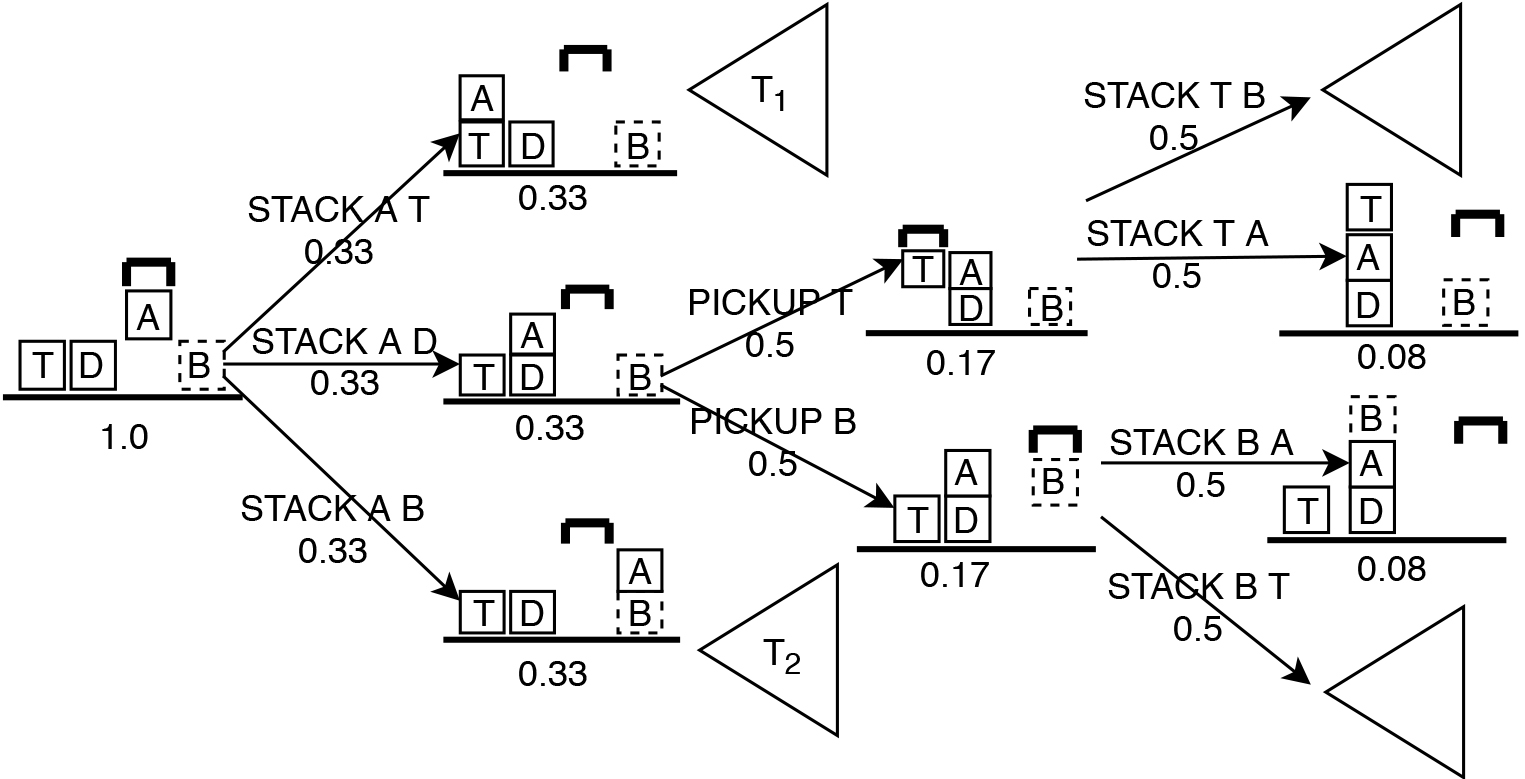
\includegraphics[width=0.6\columnwidth]{img/figure3.jpg}}
        \caption{Fragment of the decision space after PICKUP A has been proposed for block-words example in Figure \ref{fig:bw2} (B). Numbers under each state and action indicate the probability. Sub trees $T_1$ and $T_2$ are not expanded for simplicity.}
        \label{fig:feature}
\end{figure} 

\subsubsection{Risk ($R$)}
Risk quantifies the probability that the presented action will lead to \undesired.
$R$ is also coupled with the uncertainty the observer has about what the next action the user or the competitor (if present) will present. 
We model the uncertainty the observer has about the next action the user (or the competitor) presents as a uniform probability distribution across the set of applicable actions whose preconditions are satisfied in current state. 
We define $R$ as the posterior probability of reaching \undesired while the user is trying to achieve \desired. 
We extract \Suffixes from the Intervention Graph by searching breadth-first from the root until vertices containing \desired is found, including the paths in which the user has been subverted to reach \undesired. 
By construction, \desired will always be a leaf.
Let $\left | \Suffixes \right |=n$. 
The set of unsafe intervention suffixes, \SuffixesUnsafe is such that $\SuffixesUnsafe \subseteq \Suffixes$ and $\left | \SuffixesUnsafe \right |=m$ and $(m\leq n)$.
We compute posterior probability of reaching \undesired for \SuffixesUnsafe, using the chain rule in probability as, 
$Pr_{\textnormal{unsafe}}=\prod_{i=k}^{1}P(\alpha_i|\alpha_{i-1}\ldots \alpha_1)$, and $\alpha_{j} \in \lbrace\actionsTemplate{user}\rbrace$ or $\alpha_j\in\lbrace\actionsTemplate{user}\cup\actionsTemplate{other}\rbrace$ and $k$ is the length of the suffix until \undesired is reached. Then: 
\begin{equation*} 
R = \left\{\begin{matrix} \frac{\sum_{i=1}^{m}Pr_{\textnormal{unsafe}_i}}{m} & m>0\\ 0 &  m=0 \end{matrix}\right.
\end{equation*}
In Figure \ref{fig:feature}, $(n=6)$ and $(m=1)$. 
Since we assumed full observability for the observer, the root of the tree (current state) is assigned the probability of 1.0. 
Actions that are immediately possible after the current state are each assigned probabilities following a uniform distribution across the branching factor (0.33). 
Then for each applicable action in the current state, the resulting state gets the probability of ($1.0\times0.33=0.33$). 
Similarly, we apply the chain rule of probability for each following state and action level in the graph until \undesired first appears in the suffix. $R=\frac{0.08}{1}=0.08$.

\subsubsection{Desirability ($D$)}
Desirability measures the effect of the observed action to help the user pursue \desired safely.
\Suffixes is the same from $R$.
Let \SuffixesSafe be the set of suffixes that reach \desired while avoiding \undesired. Then $\SuffixesSafe =  \Suffixes\setminus\SuffixesUnsafe$.
We compute  posterior probability of reaching \desired avoiding \undesired for \SuffixesSafe, using the chain rule in probability as, $Pr_{safe}=\prod_{i=k}^{1}P(\alpha_i|\alpha_{i-1}\ldots \alpha_1)$, and $\alpha_{j} \in \lbrace\actionsTemplate{user}\rbrace$ or $\alpha_j\in\lbrace\actionsTemplate{user}\cup\actionsTemplate{other}\rbrace$ and $k$ is the length of path. Then:
\begin{equation*} 
D = \left\{\begin{matrix}
\frac{\sum_{i=1}^{|\SuffixesSafe|}Pr_{safe_i}}{|\SuffixesSafe|} & |\SuffixesSafe|>0\\ 
0 &  |\SuffixesSafe|=0
\end{matrix}\right.
\end{equation*} 
In Figure \ref{fig:feature}, there are five instances where user achieved \desired  without reaching \undesired (two in sub tree $T_1$, three in the expanded branch). Following the same approach to assign probabilities for states and actions, $D= \frac{(0.08+0.08+0.08+0.04+0.04)}{5} = 0.07$.
$R$ and $D$ are based on probabilities indicating the confidence the observer has about the next observation. 
We also use graph based distance measures: (1) distance to \undesired  ($\delta_\undesired$) and (2) distance to \desired ($\delta_\desired$). Both distances are measured in the number of edges in the paths from the root of the Intervention Graph to a state containing \desired or \undesired. 


\subsubsection{Distance to $\boldsymbol{\undesired}$ ($\delta_\undesired$)} 
This feature measures the distance to state \undesired from the current state in terms of the number of edges in the paths in \Suffixes extracted from the Intervention Graph. 
We extract \Suffixes from the Intervention Graph from the root to any vertex containing \desired, including the paths in which the user has been subverted to reach \undesired instead. 
Let $\left | \Suffixes \right |=n$. 
The set of suffixes that reach \undesired, \SuffixesUnsafe is such that $\SuffixesUnsafe \subseteq \Suffixes$ and $\left | \SuffixesUnsafe \right |=m$ and $(m\leq n)$.
We count  $s$, the number of the edges (actions) before \undesired is reached for each path in \SuffixesUnsafe and $\delta_\undesired$ is defined as the average of these distance values:
\begin{equation*} 
\delta_\undesired = \left\{\begin{matrix}
\frac{\sum_{i=1}^{m}s_i}{m} & m>0\\ 
-1 &  m=0
\end{matrix}\right.
\end{equation*} 
In this formula, $-1$ indicates that the undesirable state is not reachable from the current state. For the example problem illustrated in Figure \ref{fig:feature}, $\delta_\undesired=\frac{3}{1}=3$.

\subsubsection{Distance to $\boldsymbol{\desired}$ ($\delta_\desired$)} 
This feature measures the distance to \desired from the current state. The path set \SuffixesSafe contains action sequences that reach \desired without reaching \undesired.
We count  $t$, the number of the edges where \desired is achieved safely for a path in \SuffixesSafe. 
Then, $\delta_\desired$ is defined as the average of these distances given by the formula:
\begin{equation*} 
\delta_\desired = \left\{\begin{matrix}
\frac{\sum_{i=1}^{|\SuffixesSafe|}t_i}{|\SuffixesSafe|} & |\SuffixesSafe|>0\\ 
-1 &  |\SuffixesSafe|=0
\end{matrix}\right.
\end{equation*}
In this formula, $-1$ indicates that \desired can not be reached safely from the current state. For the example problem illustrated in Figure \ref{fig:feature}, $\delta_\desired=\left \lceil \frac{3+3+7+7+3}{5} \right \rceil=5$.


\subsubsection{Active attack landmark percentage ($\mathcal{L}_{ac}$)} 
This feature captures the criticality of the current state toward contributing to \undesired. 
As defined in Chapter~\ref{chap:ch2}, Section~\ref{sec:prpdomain}, landmarks are facts that must be true in every valid plan for a planning problem.
We used the algorithm proposed by Hoffmann et al. \citeyear{hoffman2004lm} to extract fact landmarks for the planning problem $P = \langle \domainTemplate{other}, \mathrm{u}\rangle$ or $P = \langle \domainTemplate{user}, \mathrm{u}\rangle$. 
These landmarks are referred to as \textit{attack landmarks} ($\mathcal{L}_{u}$) because they establish predicates that must be true to reach \undesired.  
Landmarks have been successfully used in deriving heuristics in Plan Recognition \cite{vered2018goalrec} and generating alternative plans \cite{bryce2014diverse}. 
We compute the percentage of active attack landmarks in the current state ($\mathcal{L}_{ac}$). 
To compute $\mathcal{L}_{ac}$ in Figure \ref{fig:feature}, we count the number of landmark predicates that have become active $(l)$ in the root of the Intervention Graph. 
Then, $\mathcal{L}_{ac}$ is given by the formula: $\mathcal{L}_{ac} = \frac{l}{\left |\mathcal{L}_{u}\right|}$. In Figure \ref{fig:feature}, $l=4$ and $\mathcal{L}_{ac}=4/10=0.4$.

For each presented action, the Intervention Graph is generated and features are computed, producing the corresponding feature vector. Landmarks for the problem are computed apriori.

\subsection{Plan Space Sampling and Plan Distance Metrics}
\label{sec:planspacesampling}
Extracting Intervention Graph features can be intractable when the graph is large, there are multiple paths reaching \desired, or multiple undesirable goals. 
Therefore, for our second method for implementing $plan(o_i,g)$ we define an additional set of features, called \textit{Sampled Features} by sampling the plan space for the observer.
If the Intervention Problem is defined for a single user, we sample the observer's plan space by using an automated planner to find solutions for $P_{\textnormal{observer}}=\langle \factsUser,\actionsUser, \initialState, g\rangle$, where $g\in\lbrace \desired,\undesired \rbrace$.
If the Intervention Problem is defined for a user and a competitor, we sample the observer's plan space by using an automated planner to find solutions for $P_{\textnormal{observer}}=\langle \factsOther,\actionsUser\cup\actionsOther, \initialState, g\rangle$, where $g\in\lbrace \desired,\undesired \rbrace$. 
Note that in this method we omit \dandu for generating plans.
Sampled plans are generated with the Top-K planner \cite{riabov2014}. 
We estimate the Risk and Desirability using plan distance metrics. The intuition is that if the actor is executing an unsafe plan, then that plan should be more similar to a sample of unsafe plans, compared to a sample of safe plans. 


For each presented action, the observer computes plan distances between a reference plan ($\pi^\prime$) and sampled plans ($\Pi^{\prime\prime}$) for both \undesired and \desired.
We follow the method proposed by Vered et al. \citeyear{vered2017} to generate the observation compatible plan by concatenating the observation history with the optimal plan that reaches \undesired (and \desired) to produce $\pi^\prime$.
 
We use the Top-K planner with K$=$50 to sample the plan space.
We use Action Set Distance (ASD), State Sequence Distance (SSD), Causal Link Distance (CLD) \cite{nguyen2012generating}, Generalized Edit Distance (GED) for sequences of states and actions \cite{sohrabi2016finding} to measure the distances between the reference plan and the sampled plans for \desired and \undesired. When an action is presented, $\pi^\prime$ is computed. 
Then, observation compatible Top-K plans are produced for \undesired and \desired separately. 
Then we compute the medians of ASD, CLD and SSD, minimum remaining actions to \undesired and \desired, minimum action GED and state GED are computed for \undesired and \desired for all $\langle$reference, sample$\rangle$ pairs. 
This produces the Sampled Feature vector for the presented action. Algorithm~\ref{alg:apx} shows the pseudo-code for computing the Sampled Feature vector.

\begin{algorithm}[ht]
%\scriptsize
        \caption{Build Sampled Feature Vector}
        \label{alg:apx}
        \begin{algorithmic}[1]
                \Require $D$, $s$, \undesired, \desired
                \State $i=0;$ $ s_{i} \gets \initialState$
                \State $prefix,suffix,\Pi^{\prime\prime}, \mathcal{V} \gets \varnothing$
                \Procedure{sampledsuffixes}{$D_1,s,\mathrm{u},\mathrm{d},O$}
                        %\State $\mathcal{L}_{u} \gets$ compute remaining landmarks for the problem $P_1\langle D_1, \mathrm{u}\rangle$
                \For{$o \in O$}
                        \State \parbox[t]{0.95\linewidth}{$prefix \gets prefix + o$}
                        \State \parbox[t]{0.95\linewidth} 
                                {$s_{i+1} \gets ((s_{i} \setminus Del(o))\cup Add(o))$}
                        \For {$ g \in \{\mathrm{u}, \mathrm{d}$\}}
                                \State \parbox[t]{0.95\linewidth}{$suffix \gets OptimalPlan(s,g)$}
                                \State \parbox[t]{0.95\linewidth}{$\pi^\prime \gets prefix + suffix$}
                                \State \parbox[t]{0.95\linewidth}{$\Pi^{\prime\prime} \gets \text{Observation compatible Top-K plans for } g$}
                                \State \parbox[t]{0.95\linewidth}{$v_1 \gets$ MedianActionSetDist$(\pi^\prime, \Pi^{\prime\prime})$}
                                \State \parbox[t]{0.95\linewidth}{$v_2 \gets$ MedianCausalLinkDist$(\pi^\prime, \Pi^{\prime\prime})$}
                                \State \parbox[t]{0.95\linewidth}{$v_3 \gets$ MedianStateSequenceDist$(\pi^\prime,\Pi^{\prime\prime})$}
                                \State \parbox[t]{0.95\linewidth}{$v_4 \gets$ MinimumRemainingDistToState $(g,\Pi^{\prime\prime})$}
                                \State \parbox[t]{0.95\linewidth}{$v_5 \gets$ MinimumActionGED $(\pi^\prime, \Pi^{\prime\prime})$}
                                \State \parbox[t]{0.95\linewidth}{$v_6 \gets$ MinimumStateGED $(\pi^\prime, \Pi^{\prime\prime})$}
                                \State $\mathcal{V}(o) \gets \lbrack v_1,v_2,v_3,v_4,v_5,v_6\rbrack $
                        \EndFor
                        %\State \parbox[t]{0.95\linewidth}{$v_7 \gets$ AchievedLandmarkHeuristic $(\mathrm{u},s_{i})$}
                        %\State $\mathcal{V}(o) \gets \mathcal{V}(o)+\{v_7\}$
                \EndFor
                \EndProcedure
        \end{algorithmic}
\end{algorithm}

\subsection{Learning When to Intervene}
\label{sec:learning-to-intervene}
We train a classifier to categorize the presented observation $o_i$ into two classes: (Yes) indicating intervention is required and (No), indicating otherwise. 
We chose Naive Bayes, K-nearest neighbors, decision tree and logistic regression classifiers from Weka~\footnote{\url{http://www.cs.waikato.ac.nz/ml/weka/}}. 
Given observations labeled as Yes/No and corresponding feature vectors as training examples, we train the classifiers with 10-fold cross validation. 
The trained model is used to predict intervention for previously unseen Intervention Problems. 
Attribute selected classifiers filter the feature vector to only select critical features. 
This step reduces complexity of the model, makes the outcome of the model easier to interpret, and reduces over-fitting. 

We generated training data from twenty Intervention Problems using the benchmark domains. We used the Blocks World domain to model competitive Intervention Problems and Ferry, EasyIPC and Navigator domains to model Standard Intervention Problems.
We restricted the number of observation traces per Intervention Problem to 100 for training the classifiers.
 
A full parameter search revealed the best parameters for the classifiers. 
The decision tree classifier is tuned to pruning confidence=0.25 and minimum number of instance per leaf=2. 
The K-nearest neighbor classifier is tuned to use k=1 and distance measure=Euclidean. 
The logistic regression classifier is tuned for ridge parameter = 1.0E-8. 
The Naive Bayes classifier is tuned with the supervised discretization=True.
%
%%%%===========================================================================================================
%%%%===========================================================================================================
\section{Evaluating Intervention Recognition}
\label{sec:evaluating-intervention}
We now discuss the accuracy of the intervention recognition solutions.
As the baseline, we compare the learning based intervention accuracy to three state-of-the-art Plan Recognition algorithms from the literature. 
Our evaluation focuses on two questions: (1) Using domain-independent features indicative of the likelihood to reach \undesired from current state, can the observer correctly recognize directly and indirectly contributing suffixes to prevent the user from reaching \undesired? and (2) How does the learning approach perform against state-of the-art Plan Recognition? 
To address the first question, we evaluated the performance of the learned model on unseen Intervention Problems.

The benchmarks consist of Blocks-words, IPC Grid, Navigator and Ferry domains. For the \textbf{Blocks-words} domain, we chose word building problems. The user and the competitor want to build different words with some common letters. 
The problems in \textbf{Blocks-1} model intervention by identifying the direct contributors ($a_{crit}$), whereas the problems in \textbf{Blocks-2} model intervention by identifying the indirect contributors ($q_{crit}$) in the Blocks-words domain.
In the \textbf{IPC grid} domain, the user moves through a grid to get from point A to B. 
Certain locked positions on the grid can be opened by picking up keys. In the \textbf{Navigator} domain, the user moves from one point on a grid to another. In IPC Grid and Navigator domains, we designated certain locations on the grid as traps. The goal of the user is to navigate to a specific point on the grid without passing through the trap. In the \textbf{Ferry} domain, a single ferry moves cars between different locations. We assigned a port as \emph{compromised}. The ferry's objective is to transport cars to specified locations without passing the compromised port. 


To evaluate our trained classifiers, we generate 3 separate test problems of 20 instances each (total of 60) 
for the benchmark domains with problems different from training instances. 
The three test instances differ from the number of blocks in the Blocks Words domain, size of grid (Navigator, IPC-Grid), accessible and inaccessible paths on the grid (Navigator, IPC-Grid), and properties of artifacts in the grid (IPC-Grid). 
For each test instance we generated 10 observation traces (total of 600 test observation traces). 


We define true-positive as the classifier correctly identifying the presented action to be in $a_{crit}$ or $q_{crit}$. 
True-negative is an instance where the classifier  correctly identifying an action as not belonging to $a_{crit}$ or $q_{crit}$. False-positives are instances where classifier incorrectly identifies an action as belonging to $a_{crit}$ or $q_{crit}$. False-negatives are instances where the classifier incorrectly identifies the presented action as not belonging to $a_{crit}$ or $q_{crit}$. 
Naturally, our test observation traces contain a large number of negatives. 
To offset the bias introduced to the classifier by the class imbalance, we report Matthews correlation coefficient (MCC) because it gives an accurate measure of the quality of a binary classification while taking into account the different class sizes.
 We also report the F-score $= \frac{tp}{tp+1/2(fp+fn)}$ for the classifiers. $tp$, $fp$, $fn$ are the number of true positives, false positives and false negatives respectively.

\begin{table}[ptb]
\resizebox{\textwidth}{!}{%
\begin{tabular}{|l|ll|ll|ll|ll|ll|l|l}
\hline
\multicolumn{1}{|c|}{\multirow{3}{*}{Domain}} & \multicolumn{6}{c|}{Naive Bayes} & \multicolumn{6}{c|}{Decision Tree} \\ \cline{2-13} 
\multicolumn{1}{|c|}{} & \multicolumn{2}{c|}{Instance 1} & \multicolumn{2}{c|}{Instance 2} & \multicolumn{2}{c|}{Instance 3} & \multicolumn{2}{c|}{Instance 1} & \multicolumn{2}{c|}{Instance 2} & \multicolumn{2}{c|}{Instance 3} \\ \cline{2-13} 
\multicolumn{1}{|c|}{} & \multicolumn{1}{l|}{F-score} & \multicolumn{1}{c|}{MCC} & \multicolumn{1}{c|}{F-score} & MCC & \multicolumn{1}{l|}{F-score} & MCC & \multicolumn{1}{l|}{F-score} & MCC & \multicolumn{1}{l|}{F-score} & MCC & F-score & \multicolumn{1}{l|}{MCC} \\ \hline
\multicolumn{13}{|c|}{Intervention Graph Method} \\ \hline
\textbf{Blocks-1} & 1 & 1 & 1 & 1 & 1 & 1 & 1 & 1 & 1 & 1 & 1 & \multicolumn{1}{l|}{1} \\ \cline{1-1}


\textbf{Blocks-2} & 1 & 1 & 1 & 1 & 1 & 1 & 1 & 1 & 1 & 1 & 1 & \multicolumn{1}{l|}{1} \\ \cline{1-1}


\textbf{EasyIPC} & 1 & 1 & 1 & 1 & 1 & 1 & 1 & 1 & 1 & 1 & 1 & \multicolumn{1}{l|}{1} \\ \cline{1-1}
\textbf{Ferry} & 1 & 1 & 1 & 1 & 1 & 1 & 1 & 1 & 1 & 1 & 1 & \multicolumn{1}{l|}{1} \\ \cline{1-1}
\textbf{Navigator} & 1 & 1 & 1 & 1 & .99 & .99 & .87 & .87 & .72 & .74 & .90 & \multicolumn{1}{l|}{.90} \\ \hline


\multicolumn{13}{|c|}{Plan Space Sampling Method} \\ \hline
\textbf{Blocks-1} & .25 & .33 & .25 & .33 & .25 & .33 & .25 & .33 & .25 & .33 & .25 & \multicolumn{1}{l|}{.33} \\ \cline{1-1}
\textbf{Blocks-2} & 1 & 1 & 1 & 1 & 1 & 1 & 1 & 1 & 0.99 & 0.99 & 1 & \multicolumn{1}{l|}{1} \\ \cline{1-1}


\textbf{EasyIPC} & 1 & 1 & 1 & 1 & 1 & 1 & 1 & 1 & 1 & 1 & 1 & \multicolumn{1}{l|}{1} \\ \cline{1-1}
\textbf{Ferry} & .34 & .33 & .32 & .31 & 0.02 & -.004 & .25 & .28 & .24 & .23 & .86 & \multicolumn{1}{l|}{.86} \\ \cline{1-1}
\textbf{Navigator} & 1 & 1 & 1 & 1 & 1 & 1 & .62 & .65 & 1 & 1 & 1 & \multicolumn{1}{l|}{1} \\ \hline
\end{tabular}%
}
\caption{F-score and MCC for predicting intervention using  Intervention Graph and plan space sampling methods for Naive Bayes and Decision Tree classifiers}
\label{tab:exactapprox1}
\end{table}


\begin{table}[ptb]
\resizebox{\textwidth}{!}{%
\begin{tabular}{|l|ll|ll|ll|ll|ll|ll|}
\hline
\multicolumn{1}{|c|}{\multirow{3}{*}{Domain}} & \multicolumn{6}{c|}{Logistic Regression} & \multicolumn{6}{c|}{K-Nearest} \\ \cline{2-13} 
\multicolumn{1}{|c|}{} & \multicolumn{2}{c|}{Instance 1} & \multicolumn{2}{c|}{Instance 2} & \multicolumn{2}{c|}{Instance 3} & \multicolumn{2}{c|}{Instance 1} & \multicolumn{2}{c|}{Instance 2} & \multicolumn{2}{c|}{Instance 3} \\ \cline{2-13} 
\multicolumn{1}{|c|}{} & \multicolumn{1}{l|}{F-score} & MCC & \multicolumn{1}{l|}{F-score} & MCC & \multicolumn{1}{l|}{F-score} & MCC & \multicolumn{1}{l|}{F-score} & MCC & \multicolumn{1}{l|}{F-score} & MCC & \multicolumn{1}{l|}{F-score} & MCC \\ \hline
\multicolumn{13}{|c|}{Intervention Graph Method} \\ \hline
\textbf{Blocks-1} & 1 & 1 & 1 & 1 & 1 & 1 & 1 & 1 & 1 & 1 & 1 & 1 \\ \cline{1-1}
\textbf{Blocks-2} & 1 & 1 & 1 & 1 & 1 & 1 & 1 & 1 & 1 & 1 & 1 & 1 \\ \cline{1-1}
\textbf{EasyIPC} & .88 & .87 & .88 & .87 & .86 & .86 & 1 & 1 & 1 & 1 & 1 & 1 \\ \cline{1-1}
\textbf{Ferry} & 1 & 1 & 1 & 1 & 1 & 1 & 1 & 1 & 1 & 1 & 1 & 1 \\ \cline{1-1}
\textbf{Navigator} & 1 & 1 & 1 & 1 & .99 & .99 & 1 & 1 & .96 & .96 & .99 & .99 \\ \hline

\multicolumn{13}{|c|}{Plan Space Sampling Method} \\ \hline
\textbf{Blocks-1} & .25 & .33 & .25 & .33 & .25 & .33 & 1 & 1 & 1 & 1 & 1 & 1 \\ \cline{1-1}
\textbf{Blocks-2} & 1 & 1 & 1 & 1 & 1 & 1 & 1 & 1 & 1 & 1 & 1 & 1 \\ \cline{1-1}

\textbf{EasyIPC} & .64 & .63 & .46 & .44 & .67 & .66 & .05 & -.04 & .04 & -.03 & .05 & -.02 \\ \cline{1-1}
\textbf{Ferry} & .31 & .32 & .23 & .22 & 1 & 1 & .33 & .40 & .13 & .15 & .81 & .82 \\ \cline{1-1}
\textbf{Navigator} & .60 & .59 & .98 & .94 & .97 & .97 & .61 & .65 & 1 & 1 & 1 & 1 \\ \hline
\end{tabular}%
}
\caption{F-score and MCC for predicting intervention using  Intervention Graph and plan space sampling methods for logistic regression and k-nearest neighbor classifiers}
\label{tab:exactapprox2}
\end{table}

\begin{table}[ptb]
\resizebox{\textwidth}{!}{%
\begin{tabular}{|l|ll|ll|ll|ll|ll|ll|ll|ll|ll|}
\hline
\multicolumn{1}{|c|}{\multirow{3}{*}{Domain}} & \multicolumn{6}{c|}{Instance 1} & \multicolumn{6}{c|}{Instance 2} & \multicolumn{6}{c|}{Instance 3} \\ \cline{2-19} 
\multicolumn{1}{|c|}{} & \multicolumn{2}{c|}{RG (LAMA)} & \multicolumn{2}{c|}{RG (HSP)} & \multicolumn{2}{c|}{GM} & \multicolumn{2}{c|}{RG (LAMA)} & \multicolumn{2}{c|}{RG (HSP)} & \multicolumn{2}{c|}{GM} & \multicolumn{2}{c|}{RG (LAMA)} & \multicolumn{2}{c|}{RG (HSP)} & \multicolumn{2}{c|}{GM} \\ \cline{2-19} 
\multicolumn{1}{|c|}{} & \multicolumn{1}{l|}{F-score} & MCC & \multicolumn{1}{l|}{F-score} & MCC & \multicolumn{1}{l|}{F-score} & MCC & \multicolumn{1}{l|}{F-score} & MCC & \multicolumn{1}{l|}{F-score} & MCC & \multicolumn{1}{l|}{F-score} & MCC & \multicolumn{1}{l|}{F-score} & MCC & \multicolumn{1}{l|}{F-score} & MCC & \multicolumn{1}{l|}{F-score} & MCC \\ \hline
\textbf{Blocks-1} & .38 & .45 & .38 & .45 & .36 & .43 & .43 & .49 & .43 & .49 & .39 & .45 & .40 & .47 & .40 & .47 & .38 & .45 \\ \cline{1-1}
\textbf{Blocks-2} & 1 & 1 & .90 & .90 & 1 & 1 & 1 & 1 & .90 & .90 & 1 & 1 & 1 & 1 & .90 & .90 & 1 & 1 \\ \cline{1-1}
\textbf{EasyIPC} & .13 & .05 & .13 & .05 & .10 & .01 & .21 & .17 & .18 & .13 & .12 & .06 & .23 & .19 & .22 & .19 & .14 & .09 \\ \cline{1-1}
\textbf{Ferry} & .17 & .18 & .22 & .20 & .10 & .08 & .23 & .22 & .11 & .06 & .15 & .09 & .15 & .17 & .47 & .52 & .21 & .34 \\ \hline
\end{tabular}%
}
\caption{F-score and Matthews Correlation Coefficient (MCC) for recognizing intervention with probabilistic goal recognition (RG) using a satisficing (LAMA) and optimal (HSP) planners goal mirroring (GM). For the Navigator domain Intervention Problems, the true-negative, false negative rates were 100\%  each. Therefore, F-score and MCC are not reported for that problem set.}
\label{tab:rgv}
\end{table}




We implemented three state-of-the art Plan Recognition algorithms to compare the accuracy of intervening by Plan Recognition to the proposed learning based intervention. 
We selected Ramirez and Geffener's probabilistic Plan Recognition algorithm \cite{ramirez2010probabilistic} (both the satisficing, and optimal implementations) and the Goal Recognition with Goal Mirroring algorithm \cite{vered2018goalrec}. 
To generate satisficing plans we used the Fast Downward planner with the FF heuristic and context-enhanced additive heuristic \cite{helmert2006}.
To generate the optimal cost plans we used the HSP planner \cite{bonet01planningas}.
For each presented action, the observer solves a Plan Recognition problem using each approach. 
We assumed uniform priors for over \undesired and \desired. 
If \undesired is the top ranked goal for the presented action, then it is flagged as requiring intervention. 
The assumption is that these algorithms must also be able to correctly identify \undesired as the most likely goal for the actions in $a_{crit}$ and $q_{crit}$. 
We used the same test data suite to evaluate accuracy.

Tables \ref{tab:exactapprox1} and ~\ref{tab:exactapprox2} shows that the classifiers trained with features from the Intervention Graph achieve high accuracy for all the domains when predicting intervention for both identifying actions in $a_{crit}$ and $q_{crit}$. 
The MCC value shows that the imbalance in class sizes does not bias the classifier. 
Low false positives and false negatives suggests that the user will not be unnecessarily interrupted. 
As expected performance degrades when we use a sampled plan space to derive features.
However, the features derived from sampling the plan space produce equally good classifiers compared to the intervention graph method, when  modeling intervention by identifying actions in $a_{crit}$ and $q_{crit}$  for the Blocks-word problems.
For the Intervention Problems modeled using the benchmark domains, we were able to find that at least one of the selected classifiers responded with very high F-score when trained using plan similarity features. 
The exception to this pattern was the Intervention Problems modeled using the Ferry domain.

Features derived from the Intervention Graph accurately recognize actions in $a_{crit}$ and $q_{crit}$ where the user has limited options available to reach the desirable goal while avoiding the undesirable state. 
Thus the classifiers perform well in recognizing critical actions in new problems. 
The sampled features rely on the learning algorithm to produce accurate results when predicting intervention. 

Comparing the results in Table \ref{tab:rgv}, learning methods outperform existing Plan Recognition algorithms when predicting intervention. 
The algorithms we selected clearly struggled to predict intervention in the Navigator domain producing many false positives and false negatives.
These results suggest that although we can adopt existing Plan Recognition algorithms to identify when the user needs intervention, it also produces a lot of false negatives and false positives in correctly identifying which state (desirable/undesirable) is most likely given the observations, especially when the desirable and undesirable plans have a lot of overlap.
Comparing recognition accuracy of Blocks-1 and Blocks-2 problems using plan recognition algorithms to intervene, we see that when the undesirable state develops over a long period of time, the plan recognition algorithms recognize the undesirable plan with high accuracy. 
In other words, if the \desired and \undesired are sufficiently distinct and are far apart in the state space, intervention by using plan recognition algorithms are as effective as our proposed learning based intervention methods in most cases.
When the desirable and undesirable states are closer, existing plan recognition algorithms produce many false positives/negatives.
This is unhelpful specially considering human users because, when the intervening agent produces may false alarms and/or miss critical events that should be intervened the human users may get frustrated and turn off intervention.
Therefore, the learning approach is better suited for intervention because the observer can target specific critical actions  and at the same time the user is given some freedom to pursue his own desirable goal.

%%%===========================================================================================================
%
%%%=====================================================================================
\section{Human-Aware Intervention}
\label{sec:human-aware}
The Human-aware Intervention Problem is a variant of the single-user intervention, so the history \historyDef consists of only accepted user actions.
However, as mentioned in Section~\ref{sec:models}, the set of projections will be empty, that is $\Suffixes = \emptyset$ because planning is less accurate for projecting what the human user may do.
This means the observer must emphasize analysis of \historyDef.
Instead of relying on projections in \Suffixes, the observer \emph{learns} the function $intervene_i$.
That is, at the presented action $o_i$ it considers only $H$, \desired, and \undesired and uses a trained machine learning algorithm to decide whether to intervene.

We introduce the Rush Hour puzzle as a benchmark in order to study how human users solve the puzzle as a planning task that require intervention.
We begin with the formal definitions of the Rush Hour puzzle.
Next, we translate the Rush Hour problem into a STRIPS planning task and through a human subject study, we allow human users solve the planning problem and collect observation traces.
We formally define the Human-aware Intervention problem and propose a solution that uses machine learning to learn properties of \historyDef to determine whether or not intervention is required.
The observer for Human-aware Intervention should offer different levels of freedom to the user.
At the lowest level of freedom, the observer will intervene just before the undesirable state. 
At increased levels of freedom, the observer offers the user enough time to recover from the undesirable situation.
Varying the level of freedom allows the observer to gradually guide the user toward \desired without directly giving away the complete solution.
We evaluate the accuracy of our learning approach using the observation traces collected from the human subject study.


 

\subsection{The Rush Hour Puzzle}
The Rush Hour puzzle is a game for ages 8 and above. Figure \ref{fig:game}A shows an initial puzzle configuration on a $6 \times 6$ grid, where cars (length 2) and trucks (length 3) are arranged. 
Vertically aligned vehicles can only move up and down and horizontal vehicles can move left and right. 
Vehicles can be moved one at a time and into adjacent empty spaces. The solution to the Rush Hour puzzle is a sequence of legal moves that transforms the initial board state shown in \ref{fig:game}A to the goal state in \ref{fig:game}B. 
For the puzzle shown in Figure \ref{fig:game}, the shortest solution has 21 moves, if the number of moves is considered as the optimizing criteria. 
If optimized for the number of vehicles moved, the puzzle can be solved optimally by moving only 8 vehicles. 
It is important to note that one can obtain different ``optimal solutions" depending on whether the number of moves is minimized,
or if the number of vehicles moved is minimized.
Humans tend not to clearly make this distinction when playing the game.
\begin{figure}[tpb]
  \centering
    	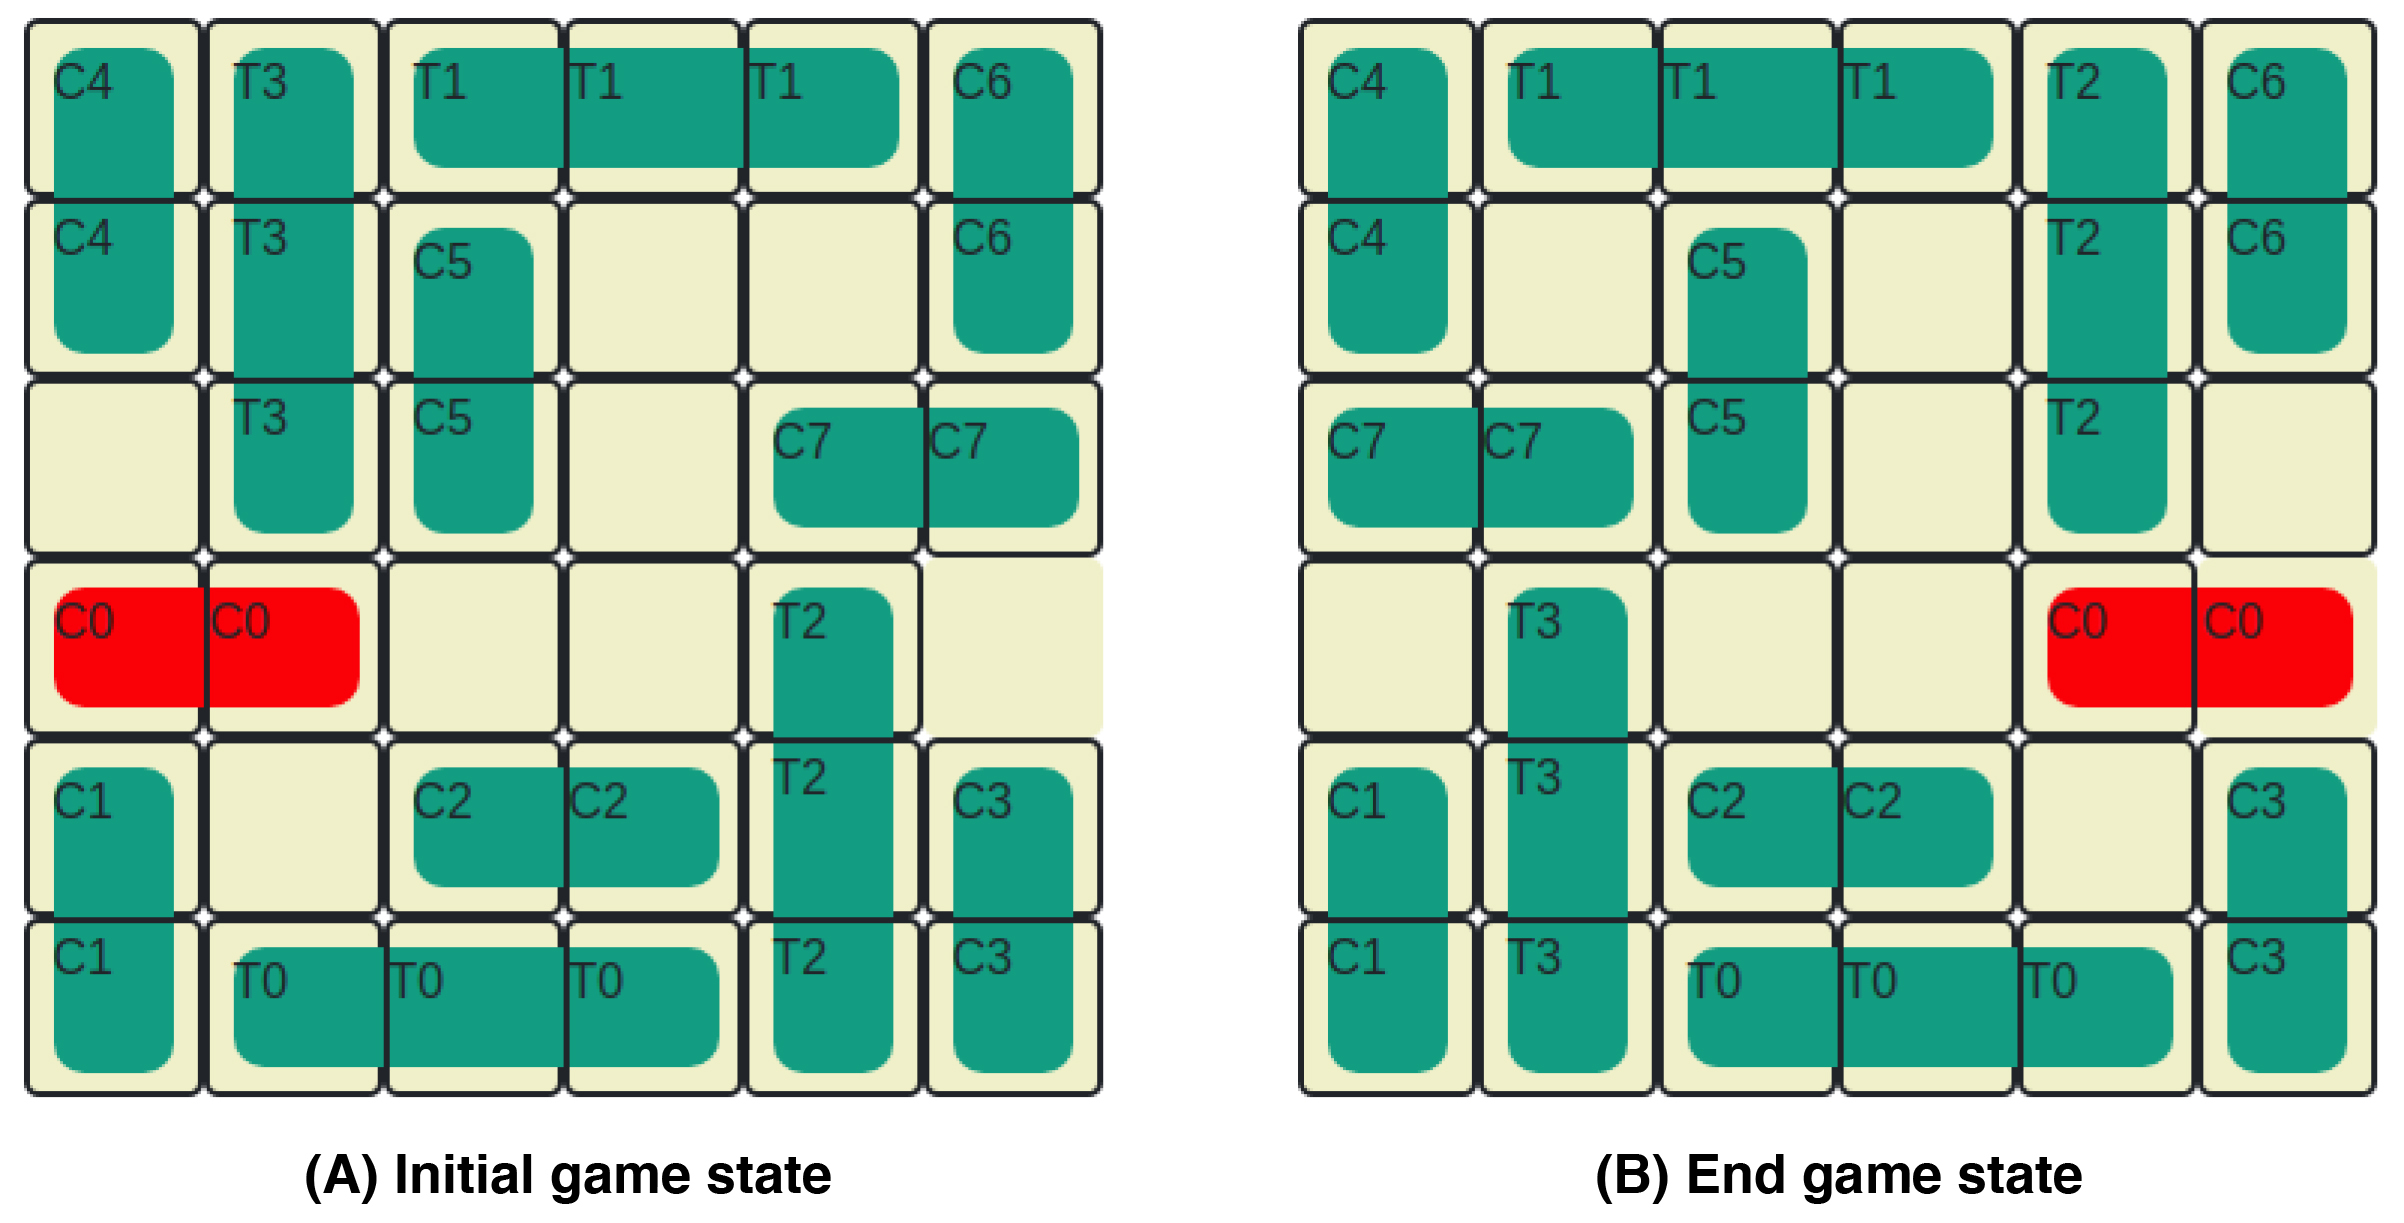
\includegraphics[width=0.7\textwidth]{img/figure4.jpg}
    	\caption{A Rush Hour instance}
    	\label{fig:game}
\end{figure}

We adopt the formal definition of a Rush Hour instance from Flake et al. \citeyear{flake2002}. 

\begin{definition} 
\label{def:rush}
A \textnormal{Rush Hour instance} is a tuple $\langle w,h,x,y,n,\mathcal{V}\rangle$ such that:
\begin{itemize}
\item $(w,h) \in {\mathbb{N}}^2$ are the grid dimensions. In the standard version, $w=h=6$
\item $(x,y), x\in\lbrace 1,w\rbrace$ and $y\in\lbrace 1,h\rbrace$ are the coordinates of the exit, which must be on the grid perimeter.
\item $n \in \mathbb{N}$ the number of non-target vehicles
\item $\mathcal{V}=\lbrace v_0, \ldots, v_n \rbrace$ is the set of $n+1$ vehicles comprised of cars $(\mathcal{C})$ and trucks $(\mathcal{T})$. Note that $|\mathcal{V}|=|\mathcal{C}|+|\mathcal{T}|$
\\$v_i \in \mathcal{C}$ is identified as $\lbrace C_0,\ldots,C_l \rbrace$, where $l=|\mathcal{C}|-1$ and $v_i \in \mathcal{T}$ is identified as $\lbrace T_0,\ldots,T_m \rbrace$, where $m=|\mathcal{T}|-1$.
\\A vehicle is a tuple $v_i=\langle x_i,y_i,o_i,s_i \rangle$, where $(x_i,y_i) \in {\mathbb{N}}^2$ are the vehicle coordinates, $o_i \in \lbrace N,E,S,W\rbrace$ is the vehicle orientation for North, East, South, West, $s_i \in \lbrace2,3\rbrace$ is the vehicle size and $C_0$ is the target vehicle.
\end{itemize}
\label{rushdef}
\end{definition}
Flake et al. \citeyear{flake2002} also defines the \textit{solution} to a Rush Hour instance as a sequence of $m$ moves, where each move consists of a vehicle identifier $i$, a direction that is consistent with the initial orientation of $v_i$, and a distance. 
Each move, in sequence must be consistent with itself and with the configuration prior to the move. 
Further, in order to move a distance $d$ the configuration must be consistent for all $d^\prime$ such that, $0\leqslant d^\prime \leqslant d$ (i.e., a vehicle can not jump over other vehicles on its path).


\subsection{The Rush Hour Puzzle as a STRIPS Planning Task for Intervention}
\label{sec:rushhourstrips}
We study how human users approach solving a cognitively engaging problem as a planning task and evaluate whether we can use domain-specific features to predict intervention. 
To collect realistic data, it is critical that the human users were willing to participate in the task. 
The Rush Hour puzzle addresses this requirement well, as evidenced by the feedback about the task we received from the demographic survey. See Section~\ref{ap:demographics} in the Appendix for details.
Although, the puzzle is a game, the environment is rich enough to simulate undesirable consequences and also offer the users a task that is challenging enough.

We translate the Rush Hour puzzle in Definition~\ref{def:rush} into a grounded STRIPS planning task $P=\langle F, A, \initialState, G\rangle$ as follows:
\begin{itemize}
\item $F=\lbrace$ 
$\lbrace \forall C_i \in \mathcal{C}$, (\texttt{car} \texttt{?}$C_i$)$\rbrace$, 
$\lbrace \forall T_i \in \mathcal{T}$, (\texttt{truck} \texttt{?}$T_i$)$\rbrace$  - for the vehicles,\\
$\lbrace \forall v_i \in \mathcal{C}\cup \mathcal{T}$ and $l_i\in \lbrace(x,y)|x\in \left[ 1..w\right ], y \in \left[ 1..h\right] \rbrace$, (\texttt{at} \texttt{?}$v_i$ \texttt{?}$l_i$)$\rbrace$ - for the vehicle positions,\\
$\lbrace \forall v_i \in \mathcal{C}\cup \mathcal{T}$ and $d_i\in \lbrace NS, SN, EW, WE \rbrace$, (\texttt{face} \texttt{?}$v_i$ \texttt{?}$d_i$)$\rbrace$ - for direction of vehicles (North to South (down), South to North (up), East to West (left), West to East (right) respectively),\\
$\lbrace \forall l_i\in \lbrace(x,y)|x\in \left[ 1..w\right ], y \in \left[ 1..h\right]\rbrace$, (\texttt{free} \texttt{?}$l_i$)$\rbrace$ - for open positions,\\
$\lbrace \forall l_i, l_j\in \lbrace(x,y)|x\in \left[ 1..w\right ], y \in \left[ 1..h\right]\rbrace$ and $d_i\in \lbrace NS, SN, EW, WE \rbrace$, (\texttt{next} \texttt{?}$d_i$ \texttt{?}$l_i$ \texttt{?}$l_j$)$\rbrace$ - for direction of the adjacent locations)
$\rbrace$

\item $A = \lbrace$\texttt{move-car} = $\langle$pre(\texttt{move-car}), add(\texttt{move-car}), del(\texttt{move-car})$\rangle \subseteq F$, \\
\texttt{move-truck} = $\langle$pre(\texttt{move-truck}), add(\texttt{move-truck}), del(\texttt{move-truck})$\rangle \subseteq F  \rbrace$
\item $\initialState \subseteq F$
\item $G = \lbrace$(\texttt{at} $C_0$ $l_i$)(\texttt{at} $C_0$ $l_j$)$\rbrace$, where $l_i=(w,3)$ and $l_j=(w-1,3)$
\end{itemize}


In order to configure the Rush Hour STRIPS planning task for intervention, we introduce an undesirable state, \undesired by designating one vehicle as \textit{forbidden}. 
The post-conditions of any action that moves the forbidden vehicle satisfies \undesired. 
The puzzle can be solved without moving the forbidden vehicle.
Therefore, moving the forbidden vehicle is also an unnecessary action, indicating that the user is exploring an unhelpful region in the state space.
Here, intervention is required to guide the user toward exploring more helpful regions in the state space.
In the Figure~\ref{fig:game}A, the forbidden vehicle is $C_2$. If the user moves $C_2$ to the left, then the board state satisfies \undesired.
The user's goal $\desired = G$.
The vehicle movement constraint introduced by the presence of the forbidden vehicle adds an extra level of difficulty to the user's planning task. 

The Rush Hour problem is also unique in that the observer is more focused on states than actions.
Recall that a history  $\historyDef = ( o_1 [s_1], o_2 [s_2], \ldots, o_{i-1} [\historyEndState])$  is a sequence of previously observed actions, which started from \initialState with the implied resulting states in brackets.
For Rush Hour, the observer relies on those implied states instead of just the actions.
For simplicity in notation, we present intervention in terms of states, although it is easy to map between actions and states because of the deterministic state transition system of the planning model.


\subsection{Domain-Specific Feature Set}
For the observer to learn $intervene_i$, we develop a set of domain-specific features for the Rush Hour problem.
We want the feature set to capture whether the user is advancing toward \desired by making helpful moves, or whether the user currently exploring a risky part in the state space and getting closer to \undesired.
We hypothesize that the behavior patterns extracted from \historyDef as features have a correlation to the event of the user moving the forbidden vehicle. 

\subsubsection{Features Based on State}
The features based on state analyze the properties of the sequence of state transitions in \historyDef from \initialState to \historyEndState $( [\initialState], [s_1], [s_2], \ldots, [\historyEndState])$.
Specifically, we look at the \textit{mobility} of the objects: target vehicle ($C_0$), the forbidden vehicle and the vehicles adjacent to the target and the forbidden vehicles.
We use the state features associated with the target vehicle to measure how close the user is to \desired. 
The state features associated with the forbidden car evaluate how close the user is to triggering \undesired. 

We manually examined the solutions produced in the human subject experiment (described later) to identify common movement patterns. 
Our analysis revealed that if the user was moving vehicles adjacent to the forbidden vehicle in such a way that the forbidden vehicle was freed, most users ended up moving the forbidden vehicle. 
Therefore, by monitoring the state changes occurring around the forbidden vehicle, we can estimate whether the user will end up moving the forbidden vehicle or not (i.e., trigger \undesired). 
Similarly, state changes occurring on the target car’s path to the exit, for example, the moves that result in reducing the number of vehicles blocking the target car is considered to be helpful to move the state closer to \desired.

\begin{figure}[tpb]
  \centering
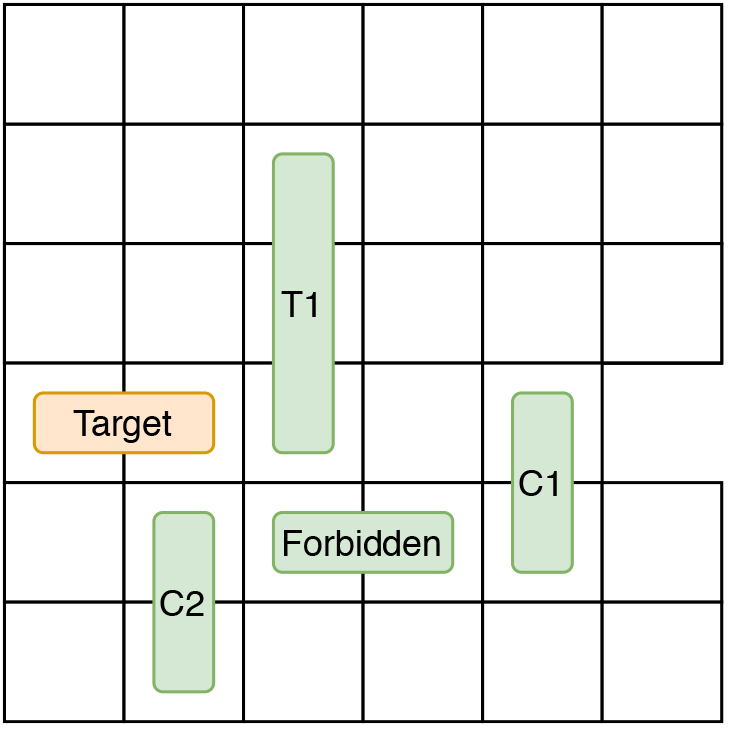
\includegraphics[width=0.25\columnwidth]{img/figure5.jpg}
  \caption{Blocker vehicles}
  \label{fig:blockers}
\end{figure}
We refer to the vehicles adjacent to the target and the forbidden vehicles as \textit{blockers} and introduce two additional object types to monitor mobility: \textit{target car blockers} and \textit{forbidden car blockers}. 
Figure~\ref{fig:blockers} illustrates an example state. 
The target car’s path is blocked by two vehicles $C_1$ and $T_1$. Therefore, target car blockers $=\lbrace C_1, T_1\rbrace$. 
We only consider the vehicles that are between the target car and the exit cell as target car blockers because, only those vehicles are preventing the target car from reaching \desired. 
The forbidden vehicle’s movement is blocked by two vehicles $C_1$ and $C_2$. 
Therefore, forbidden car blockers $=\lbrace C_1, C_2\rbrace$. 
We now describe the features based on state that are used to predict intervention in Human-aware Intervention Problems.

\begin{itemize}
\item \texttt{blocks}: number of times a move increased the number of cars blocking the target car's path
\item \texttt{frees}: number of times a move freed up empty spaces around the forbidden vehicle
\item \texttt{freebci}: number of times the number of empty spaces around the forbidden vehicle blockers increased
\item \texttt{freebcd}: number of times the number of empty spaces around the forbidden vehicle blockers decreased
\item \texttt{freegci}: number of times the number of empty spaces around the target car blockers increased
\item \texttt{freegcd}: number of times the number of empty spaces around around the target car blockers decreased
\item \texttt{mgc}: mean number of empty spaces around the target car blockers
\item \texttt{mbc}: mean number of empty spaces around the forbidden car blockers
\item \texttt{reset}: number of times the current move changed the state back to the initial puzzle configuration\\
\end{itemize}



\subsubsection{Features Based on User Actions}
The features based on user state analyze the properties of the sequence of actions from $o_1$ to $o_{i-1}$ in \historyDef $( o_1, o_2, \ldots, o_{i-1} )$
We follow the same manual analysis of solutions produced in the human subject experiment to identify common movement patterns. 
We found that the users who produce unsafe solutions often made unhelpful moves such as moving the same vehicle back and forth many times in quick succession, causing their solution to be longer compared to a safe solution. 
We statistically verified whether the relationship between the solution length and the number of forbidden vehicle moves is significant for the human subject data using Spearman's Rank Correlation Coefficient. 
The test showed that the relationship is significant (p-value $<0.05$). 
See Section~\ref{ap:lengroups} in the Appendix for a summary of raw data.

Similarly, we observed that comparing the number of moves of the user's solution to an optimal solution produced by an automated planner is helpful in identifying whether the user is moving away from \desired or making progress. 
In order to verify this observation, we use the HSP planner \cite{bonet01planningas} to find cost optimal solutions for the Rush Hour planning tasks (see Section~\ref{sec:rushhourstrips}) used in the human subject experiment.
We statistically verified that the relationship between the length difference between the user's solution and the optimal solution found by an automated planner, and the number of forbidden vehicle moves is significant using Spearman's Rank Correlation Coefficient (p-value $<0.05$).

Thus, we conclude that features derived from the length and number of backtracking moves in \historyDef can be used to predict when the user is getting close to \undesired. 
We introduce an unhelpful move called the \textit{h-step backtrack}, which is a move that takes the  state back to a previously seen state by $h$ number of steps (i.e., an undo operation).
When deriving the feature to capture backtracking moves, we only consider $h=1$, which asks the question did the observation $o_{i-1}$ undo the effect of the observation $o_{i-2}$?

We now describe the features based on actions that are used to predict intervention in Human-aware Intervention Problems.
\begin{itemize}
\item \texttt{len}: number of moves in \historyDef
\item \texttt{len-opt}: difference of the number of moves in \historyDef and the number of moves in the safe optimal solution produced by an automated planner for the same planning task.
\item \texttt{backtracks}: number of 1-step backtrack actions in \historyDef
%\item \texttt{forbidden}: number of times the forbidden vehicle is moved
%\item \texttt{first}: number of moves until the forbidden vehicle was moved for the first time in \historyDef
\item \texttt{prop}: number of moves until the forbidden vehicle was moved for the first time in \historyDef divided by the number of moves in the safe, optimal solution produced by an automated planner for the same planning task.
\item \texttt{moved}: number of vehicles moved in \historyDef
\end{itemize}

%===========================================================================================================
%%%===========================================================================================================
\section{Evaluating Human-Aware Intervention}
\label{sec:evaluating-hai}
To evaluate the efficacy of the features based on state and features based on actions in predicting intervention for Human-aware Intervention Problems, we use actual observation traces collected from a human subject study, where human users solve Rush Hour planning tasks on a Web simulator.
We generate learned models that predict intervention while offering different levels of freedom to the user. 
We consider three levels of freedom ($k=\lbrace 1,2,3 \rbrace$) for the evaluation. 
A model trained for the lowest level of freedom ($k=1$), predicts intervention one move before the undesirable state. 
This configuration offers no time for the user to recover from the undesirable state. 
A model trained for the next level of freedom ($k=2$), intervenes the user two moves before the undesirable state is satisfied and offers the user some time to take corrective action. 
A model trained for the highest level of freedom ($k=3$), intervenes the user three moves before the undesirable state.
We begin with the experiment protocol and briefly describe the findings. 
Next, we discuss the learning methods used to predict intervention. Finally, we discuss the accuracy of prediction compared to the Plan Recognition as Planning algorithm proposed by \cite{ramirez2010probabilistic}.

\subsection{Rush Hour Experiment Protocol}
\label{sec:experimentprotocol1}
We recruited subjects from a university student population. 
The sample comprised of college students in Computer Science, Psychology, Agriculture and Business majors. 
136 participants completed  the study. 
The participants were not compensated for their time. 
After obtaining informed consent, the participants were directed to the Web URL (\url{https://aiplanning.cs.colostate.edu:9080/}), which hosted the Rush Hour simulator software. 
Each participant was assigned to solve one randomly selected Rush Hour puzzle. 
We did not place any time restriction for the puzzle solving task. Participants also had the option to use an online tutorial (available on the Web simulator application) on how to play the Rush Hour puzzle. 
Each puzzle contained one forbidden vehicle. 
Once the puzzle solving task was completed, the participants were asked to complete a short demographic survey on their general puzzle solving habits. 
117 of the 136 participants also completed the demographics survey. 

When choosing Rush Hour puzzle instances for the human subject study, we want to carefully balance the puzzle’s difficulty for a human user. 
Especially, considering the PSPACE-completeness of the (generalized)
puzzle, we need the puzzles to be solvable by human users in a reasonable time. 
We used a pilot study to determine the puzzle difficulty. 
See Section~\ref{ap:pilot} in the Appendix.
We ensured that the experiment protocol fully adhered to the Rush Hour planning task definitions (Section~\ref{sec:rushhourstrips}). 
The goal of the Rush Hour planning task (\desired) is clearly communicated to the user.
To instill the importance of avoiding the forbidden vehicle in the user’s mind, we provided an information message (yellow information bar in Figure~\ref{fig:ui}) to inform about the presence of a forbidden vehicle without specifying the vehicle identifier.
The users were also informed that the puzzle can be solved without moving the forbidden vehicle. 
If the user moved the forbidden vehicle, no visual cues (error messages, blocks) were given. 
Therefore, the undesirable state (\undesired) remained hidden to the user.
To simulate discrete actions, the vehicles on the board could only be moved one cell at a time. 
The user can click on the object to select it and move it by clicking on an empty adjacent cell. 
Invalid moves (vehicle dragging and jumps) are blocked and the user is notified via an alert message. 
We record the user's solution to the STRIPS planning task as a sequence of actions in a text file.

\begin{figure}[tpb]
  \centering
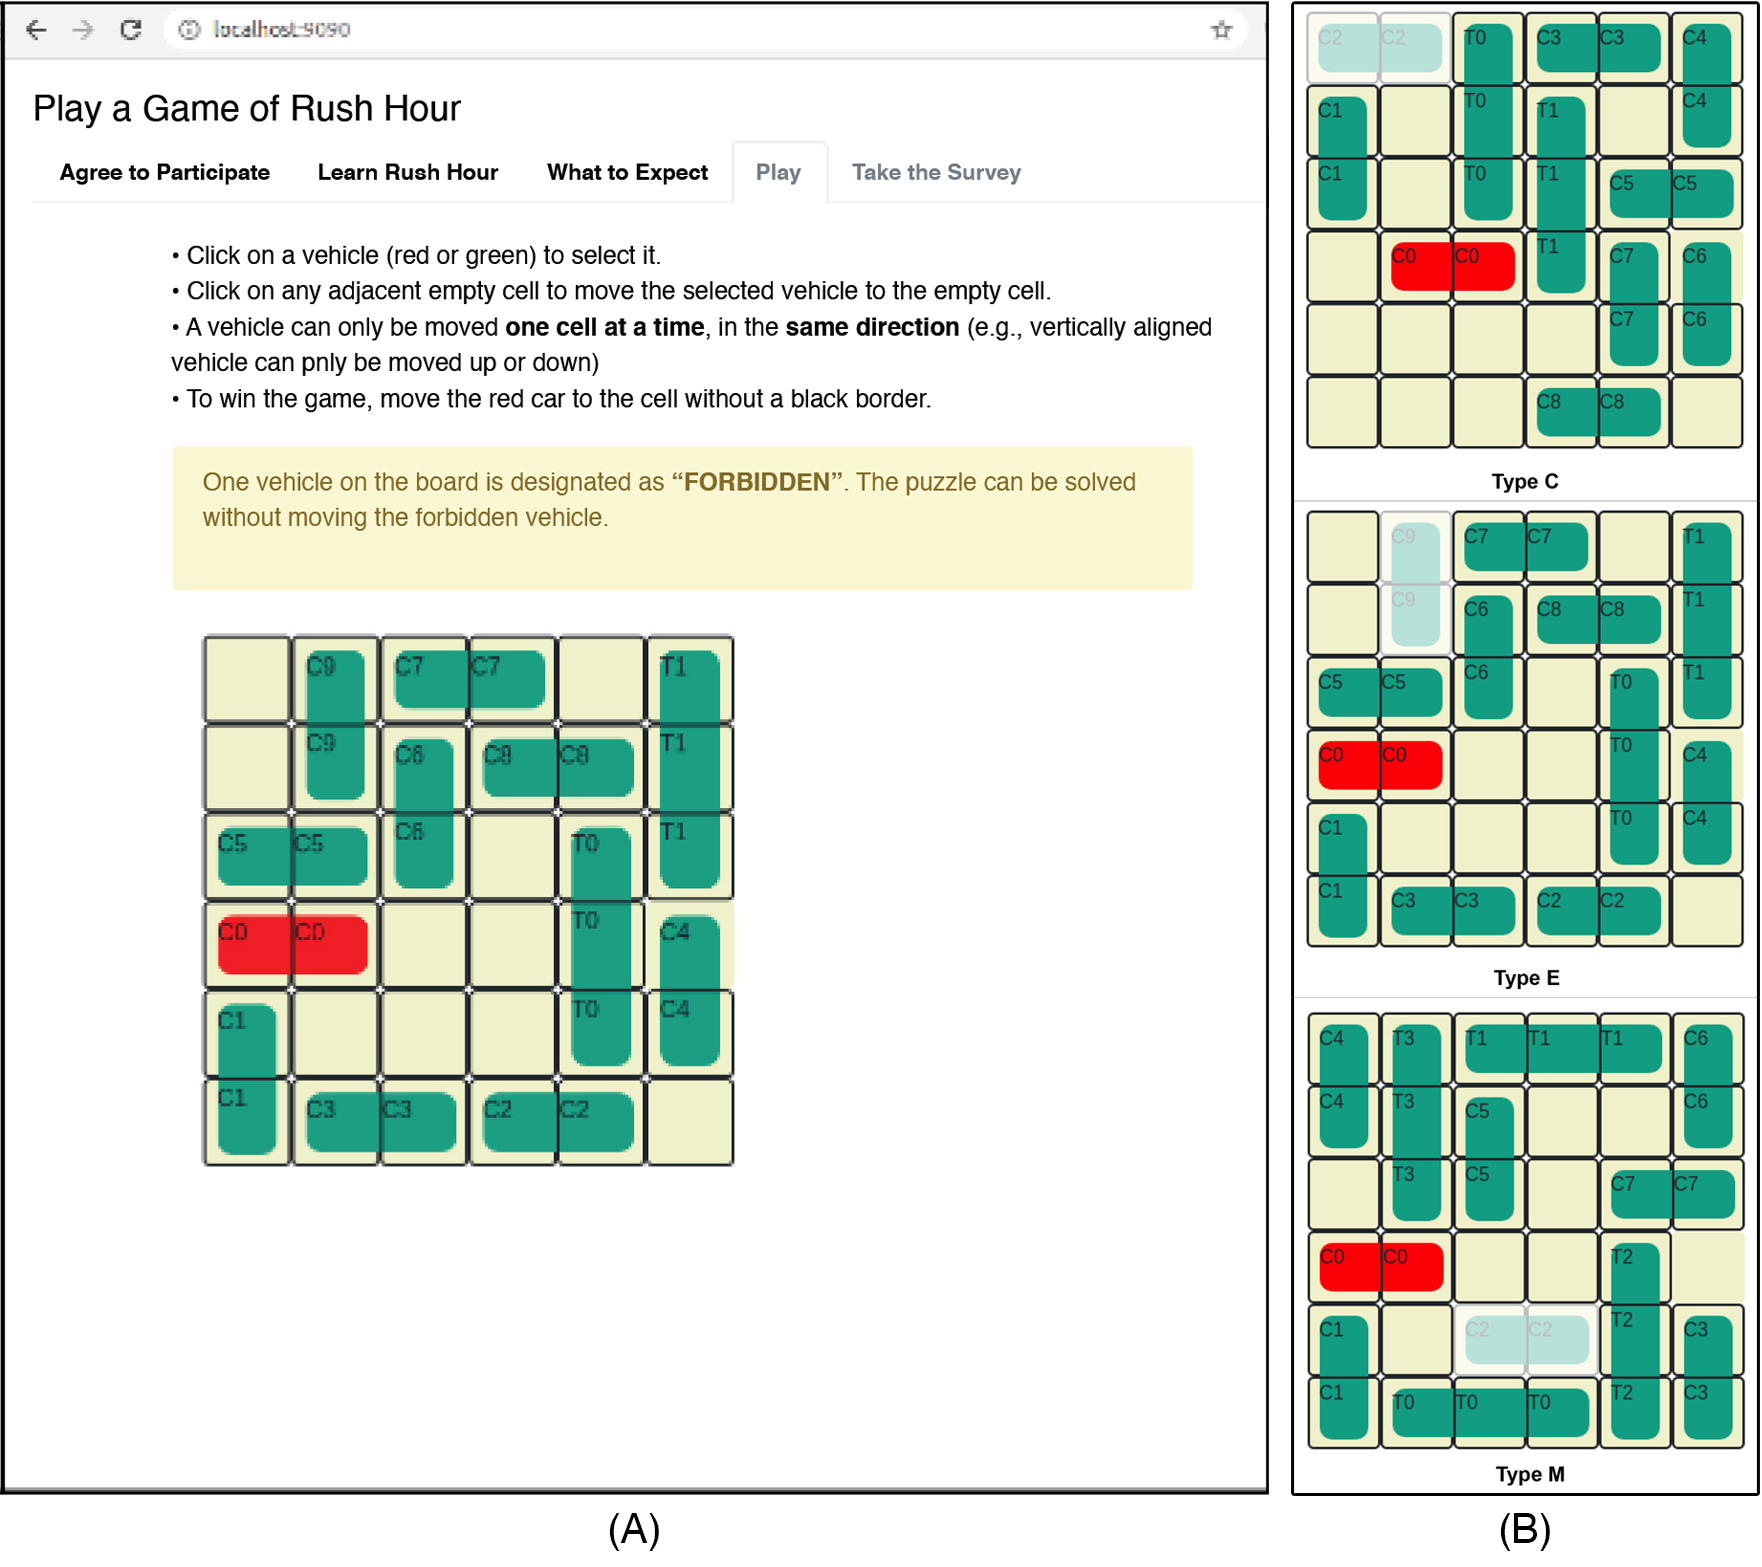
\includegraphics[width=0.8\columnwidth]{img/figure6.jpg}
  \caption{(A) Rush Hour planning task Web interface. The forbidden vehicle for this configuration is $C_9$. (B) Rush Hour puzzle configuration types with forbidden vehicles highlighted.}
  \label{fig:ui}
\end{figure}

We use ten Rush Hour planning tasks for the experiment. 
For analysis purposes (see Appendix), we separate the ten puzzles into three groups by the position of the forbidden vehicle. 
As shown in Figure~\ref{fig:ui}(B), type \textbf{C} has the forbidden vehicle in the \textbf{c}orner of the board. 
Type \textbf{E} has the forbidden vehicle on an \textbf{e}dge. 
Type \textbf{M} has the forbidden vehicle in the \textbf{m}iddle. The experiment uses four puzzles of type C, five puzzles of type E and one puzzle of type M.


\subsection{The Learning Methods}
\label{sec:learningmethods}
Our solution to the Human-aware Intervention Problem uses machine learning to predict whether \undesired will be reached in $k$ moves, given \historyDef, where $k=\lbrace 1,2,3\rbrace$.
To produce the learned models, we first partition the 136 human user solution from the experiment into training (70\%) and test (30\%) sets. 
To produce the \historyDef for a user, the user's solution is pre-processed to only include the moves until one step, two steps and three steps before the forbidden vehicle was moved for the first time. 
For example, in a  solution $O=\lbrace o_1, \ldots, o_i\rbrace$, if a user moved the forbidden vehicle in step $i$, we generate three observation traces $O_1=\lbrace o_1, \ldots, o_{i-1}\rbrace$, $O_2=\lbrace o_1, \ldots, o_{i-2}\rbrace$ and $O_3=\lbrace o_1, \ldots, o_{i-3}\rbrace$ corresponding to that user. 
Observation traces of type $O_1$ were used to train the model for $k=1$, observation traces of type $O_2$ were used to train the model for $k=2$ and so on.
Given the sequence of actions in the user's solution, the corresponding state after each move required for \historyDef is derived using the STRIPS planning model for the corresponding Rush Hour puzzle.
We use the features based on state and features based on actions together to train five classifiers with 10-fold cross validation for each value of $k$. 
We explore a number of classifiers: the decision tree, random forest, K-nearest neighbor, Logistic Regression and Naive Bayes. 
The classifiers are used in the supervised learning mode. 
We summarize the parameters used in each learning method below:
\begin{itemize}
\item \textit{Decision Tree:} We use the J48 classifier available on the WEKA platform \cite{hall09}. This classifier implements the C4.5 algorithm \cite{quinlan1993c45}. The decision tree classifier is tuned to user pruning confidence$=$0.25 and the minimum number of instances per leaf$=$2.
\item \textit{Random Forest:} This classifier is tuned to use bagging with 100 iterations and a base learner. These configuration parameters are available on the WEKA platform. 
\item \textit{k Nearest Neighbor (KNN):} We use this classifier with a Euclidean distance metric, considering the value $k=1$
\item \textit{Logistic Regression:} This classifier is tuned for ridge parameter $= 1.0E-8$.
\item \textit{Naive Bayes:} This classifier is tuned with the supervised discretization$=$\texttt{True}.
\end{itemize}


\subsubsection{Human-aware Intervention Accuracy}
We used the learned models on the test data set to predict whether the user should be intervened given \historyDef. 
In order to evaluate the classifier accuracy, we first define true-positives, true-negatives, false-positives, false-negatives for the human-aware Intervention Problem. 
A true-positive is when the classifier correctly predicts that \undesired will be reached in $k$ moves given \historyDef.
A true-negative is an instance where the classifier correctly predicts that the \undesired will not be reached in $k$ moves.
A false-positive is an instance where the classifier incorrectly identifies that the \undesired will be reached in $k$ moves.
A false-negative is an instance where the classifier identifies that the \undesired will not be reached in $k$ moves, but in fact it does.


Table~\ref{tab:rupsraccuracy} summarizes the precision, recall and F-score for predicting intervention for $k=\lbrace 1,2,3 \rbrace$. 
It can be seen that the Logistic Regression classifier performs the best with high precision/recall compared to other classifiers when predicting intervention for $\lbrace k=1,2\rbrace$
When $k=3$, the Logistic Regression classifier predicts intervention with high recall but slightly lower precision. 
The precision of the decision tree classifier improves for higher values of $k$.
However, the recall and F-score drop when $k=3$.
The Naive Bayes classifier reported the lowest precision compared to all other classifiers for any value of $k$.

\begin{table}[pbt]
\resizebox{\textwidth}{!}{%
\begin{tabular}{|l|l|l|l|l|l|l|l|l|l|}
\hline
\multicolumn{1}{|c|}{\multirow{2}{*}{Classifier}} & \multicolumn{3}{c|}{$k=1$} & \multicolumn{3}{c|}{$k=2$} & \multicolumn{3}{c|}{$k=3$} \\ \cline{2-10} 
\multicolumn{1}{|c|}{} & \multicolumn{1}{c|}{Precision} & Recall & F-score & Precision & Recall & F-score & Precision & Recall & F-score \\ \hline
Decision Tree & 0.70 & 0.90 & 0.89 & 0.80 & 0.95 & 0.87 & 0.89 & 0.81 & 0.85 \\ \cline{1-1}
Random Forest & 0.76 & 0.9 & 0.83 & 0.75 & 0.86 & 0.80 & 0.86 & 0.90 & 0.88 \\ \cline{1-1}
KNN & 0.89 & 0.76 & 0.82 & 0.86 & 0.86 & 0.86 & \textbf{0.95} & \textbf{0.90} & \textbf{0.93} \\ \cline{1-1}
Logistic Regression & \textbf{0.91} & \textbf{0.95} & \textbf{0.93} & \textbf{0.87} & \textbf{1} & \textbf{0.93} & \textbf{0.91} & \textbf{0.95} & \textbf{0.93} \\ \cline{1-1}
Naive Bayes & 0.73 & 0.90 & 0.81 & 0.74 & 0.86 & 0.83 & 0.68 & 0.90 & 0.78 \\ \hline
\end{tabular}
}%
\caption{Precision, Recall and F-scores for the prediction accuracy of the Human-aware Intervention learned models. Best values are in bold. $k$ = number of moves remaining until the forbidden vehicle is moved}
\label{tab:rupsraccuracy}
\end{table}



\subsubsection{Human-aware Intervention as a Plan Recognition Problem}
Recall that in Section~\ref{sec:distinguishing}, we showed that it is possible to frame the Intervention Problem as a Plan Recognition task, where the observer models the \undesired and \desired as the set of likely goals of the user.
Then, we can implement the observer in the Rush Hour puzzle solving task as a probabilistic Plan Recognition agent that solves the Plan Recognition Problem $T=\langle \domainUser, \mathcal{G}, \historyDef, Prob \rangle$, where \domainUser is the planning domain, the set of likely goals $\mathcal{G}=\lbrace \mathrm{u},\mathrm{d}\rbrace$, \historyDef is the observation sequence and $Prob$ is a probability distribution over $\mathcal{G}$. 
By compiling the observations away into the domain theory, Ramirez and Geffner showed that, it is possible to use an automated planner to find plans that are compatible with the observations and use these observation compatible plans to determine what the most likely goal and plan \cite{ramirez2010probabilistic} is for the user. 
They evaluated the approach on benchmark planning domains.

If the observer can recognize \undesired as the most likely goal given the observations, then the user can be intervened at that point.
We adapt the Plan Recognition as Planning (PRP) algorithm proposed by \cite{ramirez2010probabilistic}, to evaluate how the observer
executing PRP recognizes the most likely goal given the observation traces $O_1=\lbrace o_1, \ldots, o_{i-1}\rbrace$, $O_2=\lbrace o_1, \ldots, o_{i-2}\rbrace$ and $O_3=\lbrace o_1, \ldots, o_{i-3}\rbrace$, corresponding to $k=\lbrace 1,2,3\rbrace$.
We use the same test set from the classifier evaluation to evaluate the PRP algorithm in predicting intervention.
This experiment also allows us to evaluate the PRP algorithm on plans generated by human users.

In order to evaluate the PRP accuracy, we first define true-positives, true-negatives, false-positives, false-negatives for the observer implementing the PRP algorithm. 
A true-positive is when the observer correctly selects \undesired as the most likely goal given the observation traces $O_1$, $O_2$ and $O_3$ for $\lbrace k=1,2,3\rbrace$ respectively.
A true-negative is an instance where the observer correctly does not select \undesired as the most likely goal given the observation traces. 
A false-positive is an instance where the observer incorrectly identifies \undesired as the most likely goal given the observations. 
A false-negative is an instance where the observer incorrectly does not select \undesired as the most likely goal but in fact it is.

Table~\ref{tab:prp} summarizes the precision, recall and F-score for deciding to intervene correctly for $k=\lbrace 1,2,3\rbrace$ using PRP. 
PRP requires goal priors as an input to the algorithm. 
We used the Fast-Downward planner \cite{richterWestphal10.jair.LAMA} to generate satisficing plans that are compatible with the observations for PRP. 
Our assumption of the users' plans being satisficing is justified by the findings reported in Section~\ref{ap:distribution} in the Appendix. 
It shows that the majority of the users did not find optimal length solutions.
In order to analyze the algorithm performance on different goal priors, we set three levels: (1) uniform goal priors, where \undesired and \desired are equally likely (i.e., $P(\mathrm{u})=P(\mathrm{d})$), (2) \undesired is more likely and (3) \desired is more likely. 
We decided on these prior probability distributions based on the forbidden vehicle's position on initial game configurations used in the experiment. 
We set a higher value for \undesired to indicate the situation where the forbidden vehicle is not blocked by other vehicles. 
As a result, the user will likely move it. 
We set \desired as high if the forbidden vehicle is blocked in the initial configuration, to indicate that the user will be less likely to move it. 
The uniform probability is the default.

It can be seen that PRP accuracy in predicting when the \undesired will be reached is lower compared to the learned models for all levels of $k$.
The accuracy does not change with values of $k$. 
This observation is consistent with the accuracy of the logistic regression model (i.e., the best performing learned model).
When the goal priors are biased in favor of the undesirable state, the prediction accuracy slightly improves. 
However, giving a higher prior to \undesired contradicts with our intervention models' assumptions that the user wants to avoid the undesirable state, which implies that $P(\mathrm{u})$ must be low.




\begin{table}[tpb]
\resizebox{\textwidth}{!}{%
\begin{tabular}{|l|l|l|l|l|l|l|l|l|l|}
\hline
\multirow{2}{*}{Goal Priors} & \multicolumn{3}{c|}{$k=1$} & \multicolumn{3}{c|}{$k=2$} & \multicolumn{3}{c|}{$k=3$} \\ \cline{2-10} 
 & Precision & Recall & F-score & Precision & Recall & F-score & Precision & Recall & F-score \\ \hline
Uniform & 0.67 & 0.56 & 0.61 & 0.67 & 0.56 & 0.61 & 0.56 & 0.67 & 0.61 \\ \cline{1-1}
$P$(\undesired) = 2$\times P$(\desired) & 0.69 & 0.61 & 0.65 & 0.69 & 0.61 & 0.65 & 0.69 & 0.61 & 0.65 \\ \cline{1-1}
$P$(\desired) = 2$\times P$(\undesired) & 0.67 & 0.56 & 0.61 & 0.67 & 0.56 & 0.61 & 0.67 & 0.56 & 0.67 \\ \hline
\end{tabular}
}%
\caption{Precision, Recall and F-scores for solving the r-UPSR problem as a Plan Recognition problem with the Probabilistic Plan Recognition as Planning algorithm.}
\label{tab:prp}
\end{table}


%===========================================================================================================
%%===========================================================================================================
\section{Discussion}
\label{sec:discussion}
In this chapter, we formalized a family of Intervention Problems and showed that how these problems can be solved using a combination of Plan Recognition methods and classification techniques to decide when to intervene.
The Unsafe Suffix Intervention Problem uses automated planners to \textbf{project the remaining suffixes} and extract features that can differentiate unsafe remaining suffixes from the safe remaining suffixes. 
In contrast, the Human-aware Intervention Problem uses \textbf{only the observed history \historyDef} to extract features that can separate the solutions leading to undesirable state from the solutions that will avoid it.
We compared the Unsafe Suffix Intervention and Human-aware Intervention using the state-of-art Plan Recognition approaches in the literature as the baseline and found that our learning based intervention solutions dominate the existing Plan Recognition algorithms for both benchmark Intervention Problems and a new intervention benchmark, Rush Hour.

In Unsafe Suffix Intervention, when intervention models are trained using features extracted from the Intervention Graph, all the learned models chose distance to \undesired and Risk as the dominant features. We were not able to identify clear dominant features in learned models built with plan space sampling. 
In Human-aware Intervention, the best performing learned model for $k=\lbrace 1,2,3\rbrace$, the logistic regression classifier, selected  \texttt{backtracks}, \texttt{blocks}, \texttt{frees}, \texttt{reset}, \texttt{freebci}, \texttt{freebcd}, \texttt{freegci}, \texttt{freegcd}, \texttt{mgc}, \texttt{mbc} and \texttt{moved} as the features for determining intervention.

We show that both the Unsafe Suffix Intervention Problem and the Human-aware Intervention Problem can be re-framed as Plan Recognition problems and use the recognition process to decide intervention. 
The results prove the feasibility of this approach. 
However, compared to the proposed machine learning based solutions, Plan Recognition based intervention accuracy is low for both benchmark Intervention Problems and the Rush Hour Intervention Problem. 
The requirement of setting goal priors for Plan Recognition is an issue that must to be overcome for intervention. 
This is because during execution, the user's plan may be subverted to achieve the undesirable state by environmental factors (such as attackers and hidden knowledge) regardless the priors. 
In Unsafe Suffix Intervention, we find that even when we assume reasonable goal priors, if the plans for \undesired share long common action sequences with plans for \desired, Plan Recognition as Planning (PRP) approaches fail to correctly disambiguate between  \undesired and \desired. 
This affects the overall intervention accuracy by producing many false alarms and misses. 
In the intervention scenario we simulated with the Rush Hour domain, setting goal priors is even more problematic. 
This is because the user is informed about the presence of a forbidden vehicle and that the puzzle can be solved without moving it prior to executing the planning task. 
The result of that information being given to the user is that the goal prior for \undesired is low compared to \desired. 
In our experiments, we show that the recognition accuracy for PRP approach drops when goal priors are set this way. 
We remove the dependency on goal priors by using features of projected remaining suffixes (in Unsafe Suffix Recognition) and the observed partial solution \historyDef (in Human-aware Intervention) to learn the differences between safe and unsafe plans from example training data and using the learned models to predict intervention.

Our findings comparing PRP and the learned model for Human-aware Intervention show that deciding to intervene based on plan cost differences (PRP) is not sufficient, especially when intervening human users.
As seen in from the solution length distributions in Section~\ref{ap:lengroups}, the longer the human user spends exploring the state space, the higher the likelihood that his partial plan will get closer to \undesired. 
Therefore, we argue that intervention for human users require representations that capture characteristics of the actor's behavior in addition to the planning representations. 
The features based on actions and the features based on state extracted from \historyDef we propose for learning Human-aware Intervention capture the behavior patterns of the human user and as a result produce accurate learned models. 
However, a limitation of our proposed approach is that some features in the feature vector are domain-specific. 
Therefore, adopting the proposed approach in different planning domains may require feature engineering.


There are other methods one could use for generating \Suffixes, which we will explore in future work.
In Unsafe Suffix Intervention, we generated \Suffixes from the \historyEndState using an automated planner without considering the observations in \historyDef.
We then compared the suffixes in \Suffixes to an observation compatible reference plan.
\cite{ramirez2009plan, ramirez2010probabilistic, sohrabi2016plan} propose methods to compile the observations into the domain theory, which allows the planner to find observation compatible plans.
We can use this technique to also find observation compatible suffixes in \Suffixes.
By making the both \Suffixes and the reference plan compatible with the observations, we believe the plan distance features will be more accurate for the Plan Space Sampling method.



%===========================================================================================================
%%===========================================================================================================
\section{Closing Remarks}
\label{sec:closing}
Intervention is a necessity for online assistive agents and safety critical decision making, where an observer determines how to guide an user toward a desirable outcome while avoiding undesirable outcomes. 
We propose Intervention as a solution to this problem and introduced two algorithms that combine automated planning and machine learning to decide whether or not the user's likely plan will avoid the undesirable state. 
Representing the user's task as a planning problem allows us to extract features of the user's plan space that can be used to produce learned models to recognize when intervention is required. 
Our first solution Unsafe Suffix Intervention, uses automated planning to project the remaining suffixes and extract features to differentiate between safe suffixes that avoid the undesirable outcome and unsafe suffixes that do not avoid the undesirable outcome. 
The second solution, Human-aware Intervention uses only the observed plan to extract features that can differentiate between safe and unsafe solutions. 
We showed that the two learning based intervention solutions dominate the state-of-the-art Plan Recognition algorithms in identifying when intervention is required.

In this work, our objective was to identify, given a sequence of observations, whether the user requires intervention while minimizing false positives and negatives. 
For our current implementation we assumed that the intervention comes in the form of a block or an alert message. 
The natural next step following intervention is helping the user decide what to do next. 
This extension is particularly important for observers where the user is a human user who would like to be guided towards the goal instead of being given the solution outright (e.g., an automated tutoring agent). 
We identify two sub-problems in helping the user decide what to do next. 
First, we can explore how automated planning can be used to gradually probe the search space of the remaining planning task following intervention. 
In certain cases, the user may want a quick, well-focused help. 
For example, in the Rush Hour puzzle, the observer can suggest the first move in the shortest remaining plan that avoids the forbidden vehicle as a hint after intervening. 
In other cases, the user would prefer more abstract suggestion. 
For example, in the Rush Hour puzzle, the observer can suggest the vehicles that must be moved to solve the puzzle (i.e., the landmarks of the planning task). 
In various stages of the puzzle solving task, the user may opt to use these suggestions differently. 
The second sub problem is explaining intervention and the follow-up to intervention. 
We can explore how effective different explanation models (e.g., contrastive, selective) are in explaining intervention and intervention Recovery to human users.

There are several other extensions to our current intervention framework we would like to explore as future work. 
In the planning domains we used to model intervention tasks, we assumed that the user's actions are deterministic and there is only one undesirable state that needs to be avoided. 
It is possible to relax these two assumptions and explore intervention in non-deterministic environments where the user needs to avoid multiple undesirable goals. 
However, in order for intervention to be meaningful, the intervention planning domains need to be descriptive enough to model complex tasks. 
We can explore the feasibility of adopting scenario building game environments like Minecraft for this purpose.
